
%% bare_conf.tex
%% V1.4a
%% 2014/09/17
%% by Michael Shell
%% See:
%% http://www.michaelshell.org/
%% for current contact information.
%%
%% This is a skeleton file demonstrating the use of IEEEtran.cls
%% (requires IEEEtran.cls version 1.8a or later) with an IEEE
%% conference paper.
%%
%% Support sites:
%% http://www.michaelshell.org/tex/ieeetran/
%% http://www.ctan.org/tex-archive/macros/latex/contrib/IEEEtran/
%% and
%% http://www.ieee.org/

%%*************************************************************************
%% Legal Notice:
%% This code is offered as-is without any warranty either expressed or
%% implied; without even the implied warranty of MERCHANTABILITY or
%% FITNESS FOR A PARTICULAR PURPOSE! 
%% User assumes all risk.
%% In no event shall IEEE or any contributor to this code be liable for
%% any damages or losses, including, but not limited to, incidental,
%% consequential, or any other damages, resulting from the use or misuse
%% of any information contained here.
%%
%% All comments are the opinions of their respective authors and are not
%% necessarily endorsed by the IEEE.
%%
%% This work is distributed under the LaTeX Project Public License (LPPL)
%% ( http://www.latex-project.org/ ) version 1.3, and may be freely used,
%% distributed and modified. A copy of the LPPL, version 1.3, is included
%% in the base LaTeX documentation of all distributions of LaTeX released
%% 2003/12/01 or later.
%% Retain all contribution notices and credits.
%% ** Modified files should be clearly indicated as such, including  **
%% ** renaming them and changing author support contact information. **
%%
%% File list of work: IEEEtran.cls, IEEEtran_HOWTO.pdf, bare_adv.tex,
%%                    bare_conf.tex, bare_jrnl.tex, bare_conf_compsoc.tex,
%%                    bare_jrnl_compsoc.tex, bare_jrnl_transmag.tex
%%*************************************************************************


% *** Authors should verify (and, if needed, correct) their LaTeX system  ***
% *** with the testflow diagnostic prior to trusting their LaTeX platform ***
% *** with production work. IEEE's font choices and paper sizes can       ***
% *** trigger bugs that do not appear when using other class files.       ***                          ***
% The testflow support page is at:
% http://www.michaelshell.org/tex/testflow/



\documentclass[conference]{Trabalho_Final}
\usepackage{graphicx, url, epsfig, subfigure, caption, subcaption}
\usepackage{amsmath, amscd, amsthm, amsxtra}
\usepackage[T1]{fontenc}
\usepackage[brazil]{babel}   
\usepackage[latin1]{inputenc}
\usepackage{listings}
\usepackage{color}
\usepackage{verbatim}

% Some Computer Society conferences also require the compsoc mode option,
% but others use the standard conference format.
%
% If IEEEtran.cls has not been installed into the LaTeX system files,
% manually specify the path to it like:
% \documentclass[conference]{../sty/IEEEtran}





% Some very useful LaTeX packages include:2
% (uncomment the ones you want to load)


% *** MISC UTILITY PACKAGES ***
%
%\usepackage{ifpdf}
% Heiko Oberdiek's ifpdf.sty is very useful if you need conditional
% compilation based on whether the output is pdf or dvi.
% usage:
% \ifpdf
%   % pdf code
% \else
%   % dvi code
% \fi
% The latest version of ifpdf.sty can be obtained from:
% http://www.ctan.org/tex-archive/macros/latex/contrib/oberdiek/
% Also, note that IEEEtran.cls V1.7 and later provides a builtin
% \ifCLASSINFOpdf conditional that works the same way.
% When switching from latex to pdflatex and vice-versa, the compiler may
% have to be run twice to clear warning/error messages.






% *** CITATION PACKAGES ***
%
%\usepackage{cite}
% cite.sty was written by Donald Arseneau
% V1.6 and later of IEEEtran pre-defines the format of the cite.sty package
% \cite{} output to follow that of IEEE. Loading the cite package will
% result in citation numbers being automatically sorted and properly
% "compressed/ranged". e.g., [1], [9], [2], [7], [5], [6] without using
% cite.sty will become [1], [2], [5]--[7], [9] using cite.sty. cite.sty's
% \cite will automatically add leading space, if needed. Use cite.sty's
% noadjust option (cite.sty V3.8 and later) if you want to turn this off
% such as if a citation ever needs to be enclosed in parenthesis.
% cite.sty is already installed on most LaTeX systems. Be sure and use
% version 5.0 (2009-03-20) and later if using hyperref.sty.
% The latest version can be obtained at:
% http://www.ctan.org/tex-archive/macros/latex/contrib/cite/
% The documentation is contained in the cite.sty file itself.






% *** GRAPHICS RELATED PACKAGES ***
%
\ifCLASSINFOpdf
  % \usepackage[pdftex]{graphicx}
  % declare the path(s) where your graphic files are
  % \graphicspath{{../pdf/}{../jpeg/}}
  % and their extensions so you won't have to specify these with
  % every instance of \includegraphics
  % \DeclareGraphicsExtensions{.pdf,.jpeg,.png}
\else
  % or other class option (dvipsone, dvipdf, if not using dvips). graphicx
  % will default to the driver specified in the system graphics.cfg if no
  % driver is specified.
  % \usepackage[dvips]{graphicx}
  % declare the path(s) where your graphic files are
  % \graphicspath{{../eps/}}
  % and their extensions so you won't have to specify these with
  % every instance of \includegraphics
  % \DeclareGraphicsExtensions{.eps}
\fi
% graphicx was written by David Carlisle and Sebastian Rahtz. It is
% required if you want graphics, photos, etc. graphicx.sty is already
% installed on most LaTeX systems. The latest version and documentation
% can be obtained at: 
% http://www.ctan.org/tex-archive/macros/latex/required/graphics/
% Another good source of documentation is "Using Imported Graphics in
% LaTeX2e" by Keith Reckdahl which can be found at:
% http://www.ctan.org/tex-archive/info/epslatex/
%
% latex, and pdflatex in dvi mode, support graphics in encapsulated
% postscript (.eps) format. pdflatex in pdf mode supports graphics
% in .pdf, .jpeg, .png and .mps (metapost) formats. Users should ensure
% that all non-photo figures use a vector format (.eps, .pdf, .mps) and
% not a bitmapped formats (.jpeg, .png). IEEE frowns on bitmapped formats
% which can result in "jaggedy"/blurry rendering of lines and letters as
% well as large increases in file sizes.
%
% You can find documentation about the pdfTeX application at:
% http://www.tug.org/applications/pdftex





% *** MATH PACKAGES ***
%
%\usepackage[cmex10]{amsmath}
% A popular package from the American Mathematical Society that provides
% many useful and powerful commands for dealing with mathematics. If using
% it, be sure to load this package with the cmex10 option to ensure that
% only type 1 fonts will utilized at all point sizes. Without this option,
% it is possible that some math symbols, particularly those within
% footnotes, will be rendered in bitmap form which will result in a
% document that can not be IEEE Xplore compliant!
%
% Also, note that the amsmath package sets \interdisplaylinepenalty to 10000
% thus preventing page breaks from occurring within multiline equations. Use:
%\interdisplaylinepenalty=2500
% after loading amsmath to restore such page breaks as IEEEtran.cls normally
% does. amsmath.sty is already installed on most LaTeX systems. The latest
% version and documentation can be obtained at:
% http://www.ctan.org/tex-archive/macros/latex/required/amslatex/math/





% *** SPECIALIZED LIST PACKAGES ***
%
%\usepackage{algorithmic}
% algorithmic.sty was written by Peter Williams and Rogerio Brito.
% This package provides an algorithmic environment fo describing algorithms.
% You can use the algorithmic environment in-text or within a figure
% environment to provide for a floating algorithm. Do NOT use the algorithm
% floating environment provided by algorithm.sty (by the same authors) or
% algorithm2e.sty (by Christophe Fiorio) as IEEE does not use dedicated
% algorithm float types and packages that provide these will not provide
% correct IEEE style captions. The latest version and documentation of
% algorithmic.sty can be obtained at:
% http://www.ctan.org/tex-archive/macros/latex/contrib/algorithms/
% There is also a support site at:
% http://algorithms.berlios.de/index.html
% Also of interest may be the (relatively newer and more customizable)
% algorithmicx.sty package by Szasz Janos:
% http://www.ctan.org/tex-archive/macros/latex/contrib/algorithmicx/




% *** ALIGNMENT PACKAGES ***
%
%\usepackage{array}
% Frank Mittelbach's and David Carlisle's array.sty patches and improves
% the standard LaTeX2e array and tabular environments to provide better
% appearance and additional user controls. As the default LaTeX2e table
% generation code is lacking to the point of almost being broken with
% respect to the quality of the end results, all users are strongly
% advised to use an enhanced (at the very least that provided by array.sty)
% set of table tools. array.sty is already installed on most systems. The
% latest version and documentation can be obtained at:
% http://www.ctan.org/tex-archive/macros/latex/required/tools/


% IEEEtran contains the IEEEeqnarray family of commands that can be used to
% generate multiline equations as well as matrices, tables, etc., of high
% quality.




% *** SUBFIGURE PACKAGES ***
%\ifCLASSOPTIONcompsoc
%  \usepackage[caption=false,font=normalsize,labelfont=sf,textfont=sf]{subfig}
%\else
%  \usepackage[caption=false,font=footnotesize]{subfig}
%\fi
% subfig.sty, written by Steven Douglas Cochran, is the modern replacement
% for subfigure.sty, the latter of which is no longer maintained and is
% incompatible with some LaTeX packages including fixltx2e. However,
% subfig.sty requires and automatically loads Axel Sommerfeldt's caption.sty
% which will override IEEEtran.cls' handling of captions and this will result
% in non-IEEE style figure/table captions. To prevent this problem, be sure
% and invoke subfig.sty's "caption=false" package option (available since
% subfig.sty version 1.3, 2005/06/28) as this is will preserve IEEEtran.cls
% handling of captions.
% Note that the Computer Society format requires a larger sans serif font
% than the serif footnote size font used in traditional IEEE formatting
% and thus the need to invoke different subfig.sty package options depending
% on whether compsoc mode has been enabled.
%
% The latest version and documentation of subfig.sty can be obtained at:
% http://www.ctan.org/tex-archive/macros/latex/contrib/subfig/




% *** FLOAT PACKAGES ***
%
%\usepackage{fixltx2e}
% fixltx2e, the successor to the earlier fix2col.sty, was written by
% Frank Mittelbach and David Carlisle. This package corrects a few problems
% in the LaTeX2e kernel, the most notable of which is that in current
% LaTeX2e releases, the ordering of single and double column floats is not
% guaranteed to be preserved. Thus, an unpatched LaTeX2e can allow a
% single column figure to be placed prior to an earlier double column
% figure. The latest version and documentation can be found at:
% http://www.ctan.org/tex-archive/macros/latex/base/


%\usepackage{stfloats}
% stfloats.sty was written by Sigitas Tolusis. This package gives LaTeX2e
% the ability to do double column floats at the bottom of the page as well
% as the top. (e.g., "\begin{figure*}[!b]" is not normally possible in
% LaTeX2e). It also provides a command:
%\fnbelowfloat
% to enable the placement of footnotes below bottom floats (the standard
% LaTeX2e kernel puts them above bottom floats). This is an invasive package
% which rewrites many portions of the LaTeX2e float routines. It may not work
% with other packages that modify the LaTeX2e float routines. The latest
% version and documentation can be obtained at:
% http://www.ctan.org/tex-archive/macros/latex/contrib/sttools/
% Do not use the stfloats baselinefloat ability as IEEE does not allow
% \baselineskip to stretch. Authors submitting work to the IEEE should note
% that IEEE rarely uses double column equations and that authors should try
% to avoid such use. Do not be tempted to use the cuted.sty or midfloat.sty
% packages (also by Sigitas Tolusis) as IEEE does not format its papers in
% such ways.
% Do not attempt to use stfloats with fixltx2e as they are incompatible.
% Instead, use Morten Hogholm'a dblfloatfix which combines the features
% of both fixltx2e and stfloats:
%
% \usepackage{dblfloatfix}
% The latest version can be found at:
% http://www.ctan.org/tex-archive/macros/latex/contrib/dblfloatfix/




% *** PDF, URL AND HYPERLINK PACKAGES ***
%
%\usepackage{url}
% url.sty was written by Donald Arseneau. It provides better support for
% handling and breaking URLs. url.sty is already installed on most LaTeX
% systems. The latest version and documentation can be obtained at:
% http://www.ctan.org/tex-archive/macros/latex/contrib/url/
% Basically, \url{my_url_here}.




% *** Do not adjust lengths that control margins, column widths, etc. ***
% *** Do not use packages that alter fonts (such as pslatex).         ***
% There should be no need to do such things with IEEEtran.cls V1.6 and later.
% (Unless specifically asked to do so by the journal or conference you plan
% to submit to, of course. )


% correct bad hyphenation here
\hyphenation{op-tical net-works semi-conduc-tor}


\begin{document}
%
% paper title
% Titles are generally capitalized except for words such as a, an, and, as,
% at, but, by, for, in, nor, of, on, or, the, to and up, which are usually
% not capitalized unless they are the first or last word of the title.
% Linebreaks \\ can be used within to get better formatting as desired.
% Do not put math or special symbols in the title.
\title{Pedra, Papel, Tesoura, Lagarto e~\textit{Spock} }


% author names and affiliations
% use a multiple column layout for up to three different
% affiliations
%\author{\IEEEauthorblockN{Rodrigo Ferreira Guimar\~aes}
%\IEEEauthorblockA{Departamento de Ci\^encia de Computa\c{c}\~ao e Faculdade de Tecnologia\\
%Universidade de Bras\'ilia, Bras\'ilia\\
%Email: rodrigofegui@aluno.unb.br\\
%Matr\'icula: 14/0170740}
%}

\author{\IEEEauthorblockN{Diego Brian,
			  Pedro Aur\'elio e
			  Rodrigo Guimar\~aes}
\IEEEauthorblockA{Departamento de Ci\^encia de Computa\c{c}\~ao e Faculdade de Tecnologia\\
Universidade de Bras\'ilia, Bras\'ilia\\
E-mails: diegobleite@hotmail.com, pedro.almeidabsb@gmail.com e rodrigofegui@aluno.unb.br\\
Matr\'iculas: 14/0136371, 14/0158103 e 14/0170740}
}

% conference papers do not typically use \thanks and this command
% is locked out in conference mode. If really needed, such as for
% the acknowledgment of grants, issue a \IEEEoverridecommandlockouts
% after \documentclass

% for over three affiliations, or if they all won't fit within the width
% of the page, use this alternative format:
% 
%\author{\IEEEauthorblockN{Michael Shell\IEEEauthorrefmark{1},
%Homer Simpson\IEEEauthorrefmark{2},
%James Kirk\IEEEauthorrefmark{3}, 
%Montgomery Scott\IEEEauthorrefmark{3} and
%Eldon Tyrell\IEEEauthorrefmark{4}}
%\IEEEauthorblockA{\IEEEauthorrefmark{1}School of Electrical and Computer Engineering\\
%Georgia Institute of Technology,
%Atlanta, Georgia 30332--0250\\ Email: see http://www.michaelshell.org/contact.html}
%\IEEEauthorblockA{\IEEEauthorrefmark{2}Twentieth Century Fox, Springfield, USA\\
%Email: homer@thesimpsons.com}
%\IEEEauthorblockA{\IEEEauthorrefmark{3}Starfleet Academy, San Francisco, California 96678-2391\\
%Telephone: (800) 555--1212, Fax: (888) 555--1212}
%\IEEEauthorblockA{\IEEEauthorrefmark{4}Tyrell Inc., 123 Replicant Street, Los Angeles, California 90210--4321}}




% use for special paper notices
%\IEEEspecialpapernotice{(Invited Paper)}




% make the title area
\maketitle

% As a general rule, do not put math, special symbols or citations
% in the abstract
%\begin{abstract}
%O resumo vem aqui.
%\end{abstract}

% no keywords




% For peer review papers, you can put extra information on the cover
% page as needed:
% \ifCLASSOPTIONpeerreview
% \begin{center} \bfseries EDICS Category: 3-BBND \end{center}
% \fi
%
% For peerreview papers, this IEEEtran command inserts a page break and
% creates the second title. It will be ignored for other modes.
\IEEEpeerreviewmaketitle


%%%%%%%%%%%%%%%%%%%%%%%%%%%%%%%%%%%%%%%%%%%%%%%%%%%%%%%%%%%%%%%%%%%%%%%%%%%%%
\section{Introdu\c{c}\~ao}
  \label{intro}
%%%%%%%%%%%%%%%%%%%%%%%%%%%%%%%%%%%%%%%%%%%%%%%%%%%%%%%%%%%%%%%%%%%%%%%%%%%%%
Este trabalho visa fixar os conceitos aprendendido aos longo de um semestre de aulas. Para atingir tal objetivo foi desenvolvido um programa que realiza a detec\c{c}\~ao de gestos manuais, de forma a implementar o jogo popular:~\textbf{Pedra, Papel, Tesoura, Lagarto e~\textit{Spock}}~\cite{jogo}.
 
\hfill 04 de dezembro, 2015


% An example of a floating figure using the graphicx package.
% Note that \label must occur AFTER (or within) \caption.
% For figures, \caption should occur after the \includegraphics.
% Note that IEEEtran v1.7 and later has special internal code that
% is designed to preserve the operation of \label within \caption
% even when the captionsoff option is in effect. However, because
% of issues like this, it may be the safest practice to put all your
% \label just after \caption rather than within \caption{}.
%
% Reminder: the "draftcls" or "draftclsnofoot", not "draft", class
% option should be used if it is desired that the figures are to be
% displayed while in draft mode.
%
%\begin{figure}[!t]
%\centering
%\includegraphics[width=2.5in]{myfigure}
% where an .eps filename suffix will be assumed under latex, 
% and a .pdf suffix will be assumed for pdflatex; or what has been declared
% via \DeclareGraphicsExtensions.
%\caption{Simulation results for the network.}
%\label{fig_sim}
%\end{figure}

% Note that IEEE typically puts floats only at the top, even when this
% results in a large percentage of a column being occupied by floats.


% An example of a double column floating figure using two subfigures.
% (The subfig.sty package must be loaded for this to work.)
% The subfigure \label commands are set within each subfloat command,
% and the \label for the overall figure must come after \caption.
% \hfil is used as a separator to get equal spacing.
% Watch out that the combined width of all the subfigures on a 
% line do not exceed the text width or a line break will occur.
%
%\begin{figure*}[!t]
%\centering
%\subfloat[Case I]{\includegraphics[width=2.5in]{box}%
%\label{fig_first_case}}
%\hfil
%\subfloat[Case II]{\includegraphics[width=2.5in]{box}%
%\label{fig_second_case}}
%\caption{Simulation results for the network.}
%\label{fig_sim}
%\end{figure*}
%
% Note that often IEEE papers with subfigures do not employ subfigure
% captions (using the optional argument to \subfloat[]), but instead will
% reference/describe all of them (a), (b), etc., within the main caption.
% Be aware that for subfig.sty to generate the (a), (b), etc., subfigure
% labels, the optional argument to \subfloat must be present. If a
% subcaption is not desired, just leave its contents blank,
% e.g., \subfloat[].


% An example of a floating table. Note that, for IEEE style tables, the
% \caption command should come BEFORE the table and, given that table
% captions serve much like titles, are usually capitalized except for words
% such as a, an, and, as, at, but, by, for, in, nor, of, on, or, the, to
% and up, which are usually not capitalized unless they are the first or
% last word of the caption. Table text will default to \footnotesize as
% IEEE normally uses this smaller font for tables.
% The \label must come after \caption as always.
%
%\begin{table}[!t]
%% increase table row spacing, adjust to taste
%\renewcommand{\arraystretch}{1.3}
% if using array.sty, it might be a good idea to tweak the value of
% \extrarowheight as needed to properly center the text within the cells
%\caption{An Example of a Table}
%\label{table_example}
%\centering
%% Some packages, such as MDW tools, offer better commands for making tables
%% than the plain LaTeX2e tabular which is used here.
%\begin{tabular}{|c||c|}
%\hline
%One & Two\\
%\hline
%Three & Four\\
%\hline
%\end{tabular}
%\end{table}


% Note that the IEEE does not put floats in the very first column
% - or typically anywhere on the first page for that matter. Also,
% in-text middle ("here") positioning is typically not used, but it
% is allowed and encouraged for Computer Society conferences (but
% not Computer Society journals). Most IEEE journals/conferences use
% top floats exclusively. 
% Note that, LaTeX2e, unlike IEEE journals/conferences, places
% footnotes above bottom floats. This can be corrected via the
% \fnbelowfloat command of the stfloats package.

%%%%%%%%%%%%%%%%%%%%%%%%%%%%%%%%%%%%%%%%%%%%%%%%%%%%%%%%%%%%%%%%%%%%%%%%%%%%%
\section{Embasamento Te\'orico}
  \label{sec:teorico}
%%%%%%%%%%%%%%%%%%%%%%%%%%%%%%%%%%%%%%%%%%%%%%%%%%%%%%%%%%%%%%%%%%%%%%%%%%%%%
Para que haja um correto entendimento sobre o desenvolvimento deste projeto \'e importante abordar alguns aspectos relevantes, como as defini\c{c}\~oes: de uma imagem; das rela\c{c}\c{c}\~oes b\'asicas entre~\textit{pixels}: adjac\^encia, conectividade, regi\~ao e contorno; do espa\c{c}o de cor YCbCr; opera\c{c}\~oes morfol\'oligas; segmenta\c{c}\~ao, dentre outras coisas.

%%%%%%%%%%%%%%%%%%%%%%%%%%%%%%%%%%%%%%%
\subsection{Imagem e~\textit{Pixels}}
  \label{subsec:imagens}
%%%%%%%%%%%%%%%%%%%%%%%%%%%%%%%%%%%%%%%
Uma imagem pode ser definida como uma fun\c{c}\~ao bidimensional do tipo $f(x,y)$, onde $x$ e $y$ s\~ao as coordenadas espaciais e a amplitude de $f$ em qualquer ponto de coordenadas $(x,y)$ \'e denominado de intensidade da imagem naquele ponto. Quando $x$, $y$ e $f$ s\~ao valores~\textit{finitos} e~\textit{discretos}, a imagem \'e denominada imagem digital, tendo esta signific\^ancia aos computadores digitais. Um dado elemento com coordenadas $(x,y)$ e intensidade $f$ \'e denominado de~\textit{pixel}~(picture element ou, em portugu\^es, elemento de imagem), dessa forma, entende-se que uma imagem \'e constituida por um ou mais~\textit{pixels}.

Para a manipula\c{c}\~ao dos~\textit{pixels} \'e necess\'ario saber as rela\c{c}\~oes b\'asicas entre eles, como, por exemplo, a vizinhan\c{c}a. Os conceito a serem apresentados consideram uma imagem em n\'ivel de cinza.

Cada~\textit{pixel} $p$ pode possui tr\^es tipos de vizinhan\c{c}a, semelhantes a Rosa-dos-Ventos da Figura~\ref{fig:rosadosventos}:~\textit{vizinhan\c{c}a de 4},~\textit{vizinhan\c{c}a diagonal} e~\textit{vizinhan\c{c}a de 8}; onde para o primeiro, denonato por $N_4(p)$, s\~ao considerados os quatro vizinhos horizontais e verticais, seguindo as orienta\c{c}\~oes~\textit{N-S-L-O} da Rosa-dos-Ventos; para o segundo, denonato por $N_D(p)$, s\~ao considerados os vizinhos das diagonais, seguindo as orienta\c{c}\~oes~\textit{NE-SE-SO-NO}; enquanto que o terceiro tipo, denonato por $N_8(p)$, \'e a jun\c{c}\~ao dos dois anteriores.

\begin{figure}[!t]
  \centering
  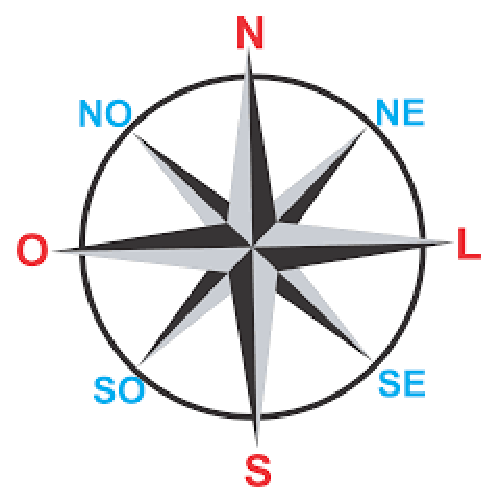
\includegraphics[width = 3 cm]{rosadosventos}
  \caption{Sinaliza\c{c}\~ao dos sentido cardeias da Rosa-dos-Ventos. Fonte~\cite{rosadosventos}.}
  \label{fig:rosadosventos}
\end{figure}

%%%%%%%%%%%%%%%%%%%%%%%%%%%%%%%%%%%%%%%
\subsection{Rela\c{c}\~oes B\'asicas entre~\textit{Pixels}}
  \label{subsec:relacaopix}
%%%%%%%%%%%%%%%%%%%%%%%%%%%%%%%%%%%%%%%
Com o conceito de vizinhan\c{c}a constru\'ido \'e poss\'ivel entender o conceito de adjac\^encia, entre dois~\textit{pixels} $p$ e $q$, que, tamb\'em, possui tr\^es tipos, sendo eles: \textbf{a) Adjac\^encia de 4}: os dois~\textit{pixels} s\~ao adjacentes de 4 se ambos possuirem o mesmo n\'ivel de cinza e se $q$ est\'a na $N_4(p)$;~\textbf{b) Adjac\^encia de 8}: os dois~\textit{pixels} s\~ao adjacentes de 4 se ambos possuirem o mesmo n\'ivel de cinza e se $q$ est\'a na $N_8(p)$;~\textbf{c) Adjac\^encia de~\textit{m}}: os dois~\textit{pixels} s\~ao adjacentes de~\textit{m} se ambos possuirem o mesmo n\'ivel de cinza e se respeitarem as condi\c{c}\~oes:~\textbf{c.1)} $q$ est\'a na $N_4(p)$ ou~\textbf{c.2)} $q$ est\'a na $N_D(p)$ e n\~ao h\'a interse\c{c}\~ao entre a $N_4(p)$ e $N_4(q)$.

Considerando um subconjunto $S$ de imagem, dois~\textit{pixels} pertencentes a $S$ s\~ao conectados, considerando um dos crit\'erios de adjac\^encia, caso exista um caminho entre eles que tamb\'em perten\c{c}a a $S$. Para qualquer~\textit{pixel} $p$ em $S$, o conjunto de~\textit{pixels} que proporciona a uni\~ao a $q$ \'e denominado de~\textit{conjunto conectado}. Caso $q$ seja adjacente a $p$, este \'e chamado de~\textit{componente conectado}.

Uma regi\~ao $R$ \'e definida como um conjunto conectado e o contorno $C$ de $R$ \'e definido como sendo os~\textit{pixels} que possuem vizinhos que tanto pertencem $R$ como n\~ao pertencente.

%%%%%%%%%%%%%%%%%%%%%%%%%%%%%%%%%%%%%%%
\subsection{Espa\c{c}o de Cores}
  \label{subsec:cores}
%%%%%%%%%%%%%%%%%%%%%%%%%%%%%%%%%%%%%%%
As imagens coloridas s\~ao constru\'idas atrav\'es de espa\c{c}os de cores, por exemplo o~\textit{RGB} (\textit{Red, Green e Blu} ou, em portugu\^es, Vermelho, Verde e Azul). Os monitores de computadores e~\textit{smartphones}, al\'em dos televisores, s\~ao constituidos por v\'arios~\textit{pixels}, como demostrado na Figura~\ref{fig:monitorpixel}, sendo que cada~\textit{pixel} \'e constituido por $3$~\textit{LEDs}, basicamente, para cada cor do~\textit{RGB}.

Considerando que cada~\textit{pixel} em cada plano de um espa\c{c}o de cores \'e descrito por $1$~\textit{byte} ou $8$~\textit{bits}; ao implementar este conhecimento no espa\c{c}o de cores~\textit{RGB} \'e poss\'ivel ter $256^3$ cores diferentes. Mesmo tendo esta grande gama de cores \'e sabido que o olho humano \'e mais sens\'ivel \`a lumin\^ancia (brilho) do que \`a cor; considerando que o RGB, em que a lumin\^ancia est\'a espalhada pelas componentes, n\~ao \'e adaptado para se aproximar da sensibilidade humanda \'e preciso utilizar outro espa\c{c}o de cores que fa\c{c}a tal adapta\c{c}\~ao.

Como op\~ao tem o espa\c{c}o de cores~\textit{YCbCr} que possui as componentes: lumin\^ancia (Y) e as cromin\^ancias (Cb e Cr), onde a lumin\^ancia \'e mais significativa do que as cromin\^ancias. \'E importante ressaltar que, devido \`a constitui\c{c}\~ao dos monitores, e similares, \'e necess\'ario que haja formas de convers\~ao entre os espa\c{c}os de cores, independente de qual seja o escolhido, para o padr\~ao~\textit{RGB}; \'e poss\'ivel tal convers\~ao entre o~\textit{RGB} e o~\textit{YCbCr}.

\begin{figure}[]
  \centering
  
\includegraphics[width = 3.5 cm]{monitorpixel}
  \caption{Aproxima\c{c}\~ao num monitor, sendo poss\'ivel perceber os~\textit{pixels} e os~\textit{LED} do espa\c{c}o de cor~\textit{RGB}. Fonte~\cite{monitor}.}
  \label{fig:monitorpixel}
\end{figure}

%%%%%%%%%%%%%%%%%%%%%%%%%%%%%%%%%%%%%%%
\subsection{Opera\c{c}\~oes Morfol\'ogicas}
  \label{subsec:morfo}
%%%%%%%%%%%%%%%%%%%%%%%%%%%%%%%%%%%%%%%  
A morfologia, geralmente, \'e considerada apenas como uma especializa\c{c}\~ao da biologia que trabalha com a forma e a estrutura dos seres vivos. Al\'em desse conceito, h\'a a morfologia matem\'atica que estuda o processamento e an\'alise de estruturas geom\'etricas. Dessa forma, tem que para o processamento de imagens \'e aplicado a morfologia matem\'atica, pois dessa forma \'e realizada a extra\c{c}\~ao de regi\~oes de uma imagem, representa\c{c}\~ao e descri\c{c}\~ao das formas de uma determinada regi\~ao.

Dessa forma, considerando imagens bin\'arias, tem-se algunas opera\c{c}\~oes, sendo elas: eros\~ao; dilata\c{c}\~ao; fechamento; abertura;~\textit{top-hat};~\textit{bottom-hat}; dentre outras, sendo que algumas destas ser\~ao exploradas neste projeto.

%%%%%%%%%%%%%%%%%%%
\subsubsection{Eros\~ao}
  \label{subsubsec:erosao}
%%%%%%%%%%%%%%%%%%%
A eros\~ao \'e definida como sendo:
$$ A \ominus B  = \{z \mid (B)_z \subseteq A\},$$
ou seja, a eros\~ao de $A$ por $B$ \'e o conjunto de todos os pontos $z$, tal que $B$ transladado de $z$ est\'a contido em $A$, como demonstrado na Figura~\ref{fig:erosao} ($B$ \'e chamado~\textit{elemento estruturante}). Dessa forma ao considerar que $B$ n\~ao tem elementos comuns com o fundo \'e poss\'ivel reescrever como sendo:
$$ A \ominus B  = \{z \mid (B)_z \cap A{^c} = \emptyset \}.$$

\begin{figure}[]
  \centering
  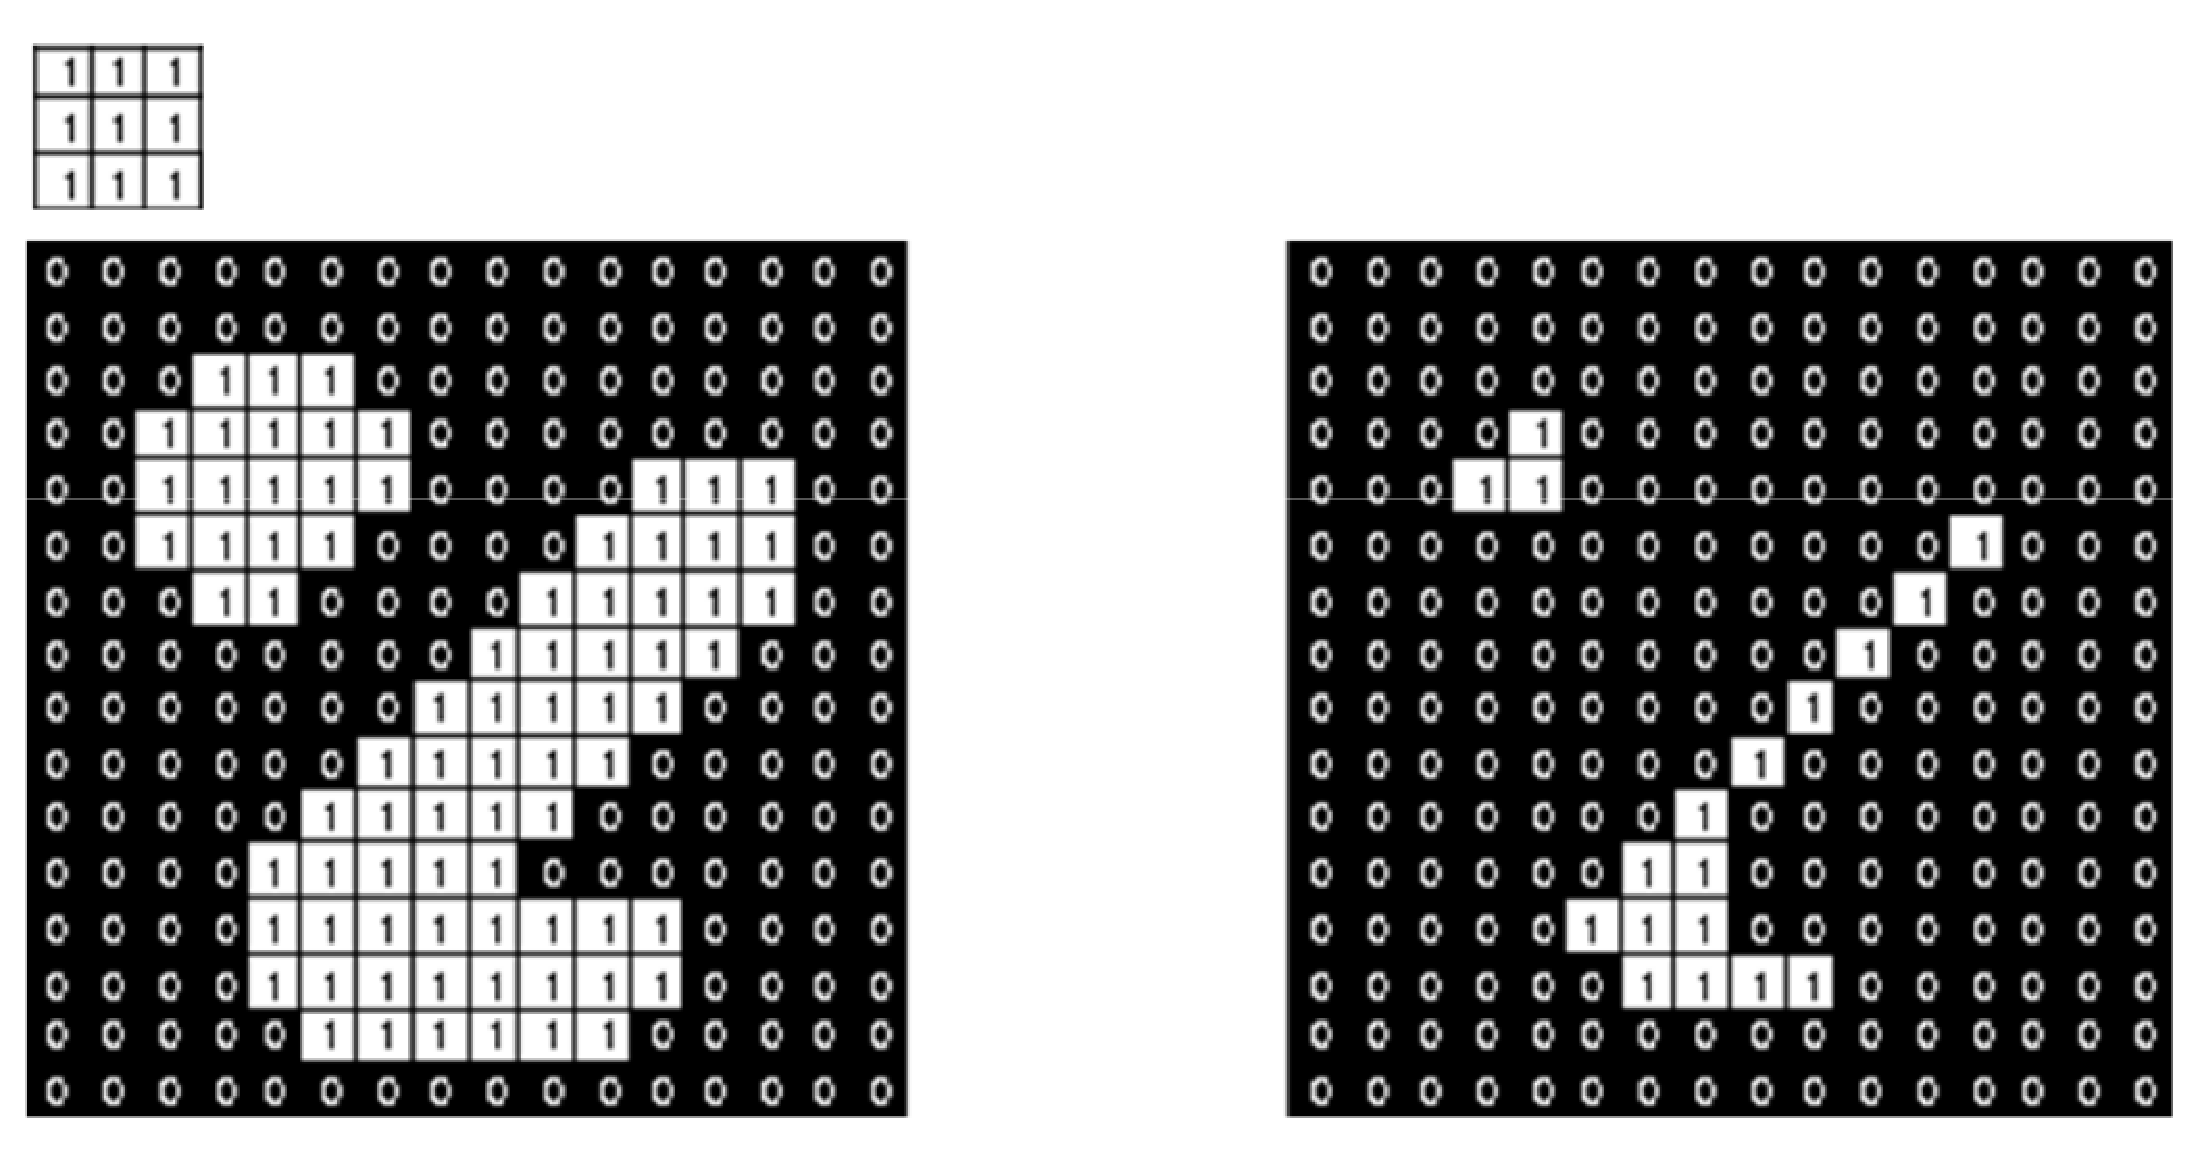
\includegraphics[width = 5 cm]{Erosao}
  \caption{Exemplo da opera\c{c}\~ao morfol\'ogica: Eros\~ao. \`A esquerda \'e a imagem original, \`a direita \'e a imagem erudida. Fonte: fornecido pelo professor.}
  \label{fig:erosao}
\end{figure}

%%%%%%%%%%%%%%%%%%%
\subsubsection{Dilata\c{c}\~ao}
  \label{subsubsec:dilatacao}
%%%%%%%%%%%%%%%%%%%
A dilata\c{c}\~ao \'e definida como sendo:
$$ A \oplus B  = \{z \mid (\hat{B})_z \cap A \neq \emptyset \},$$
ou seja, a dilata\c{c}\~ao de $A$ por $B$ \'e o conjunto de todos os deslocamentos $z$ de forma que $B$ e $A$ se sobrep\~oem, em pelo menos, por um elemento, como demonstrado na Figura~\ref{fig:dilata}; um modo alternativo:
$$ A \oplus B  = \{z \mid [(\hat{B})_z \cap A] \subseteq A \}.$$

\begin{figure}[]
  \centering
  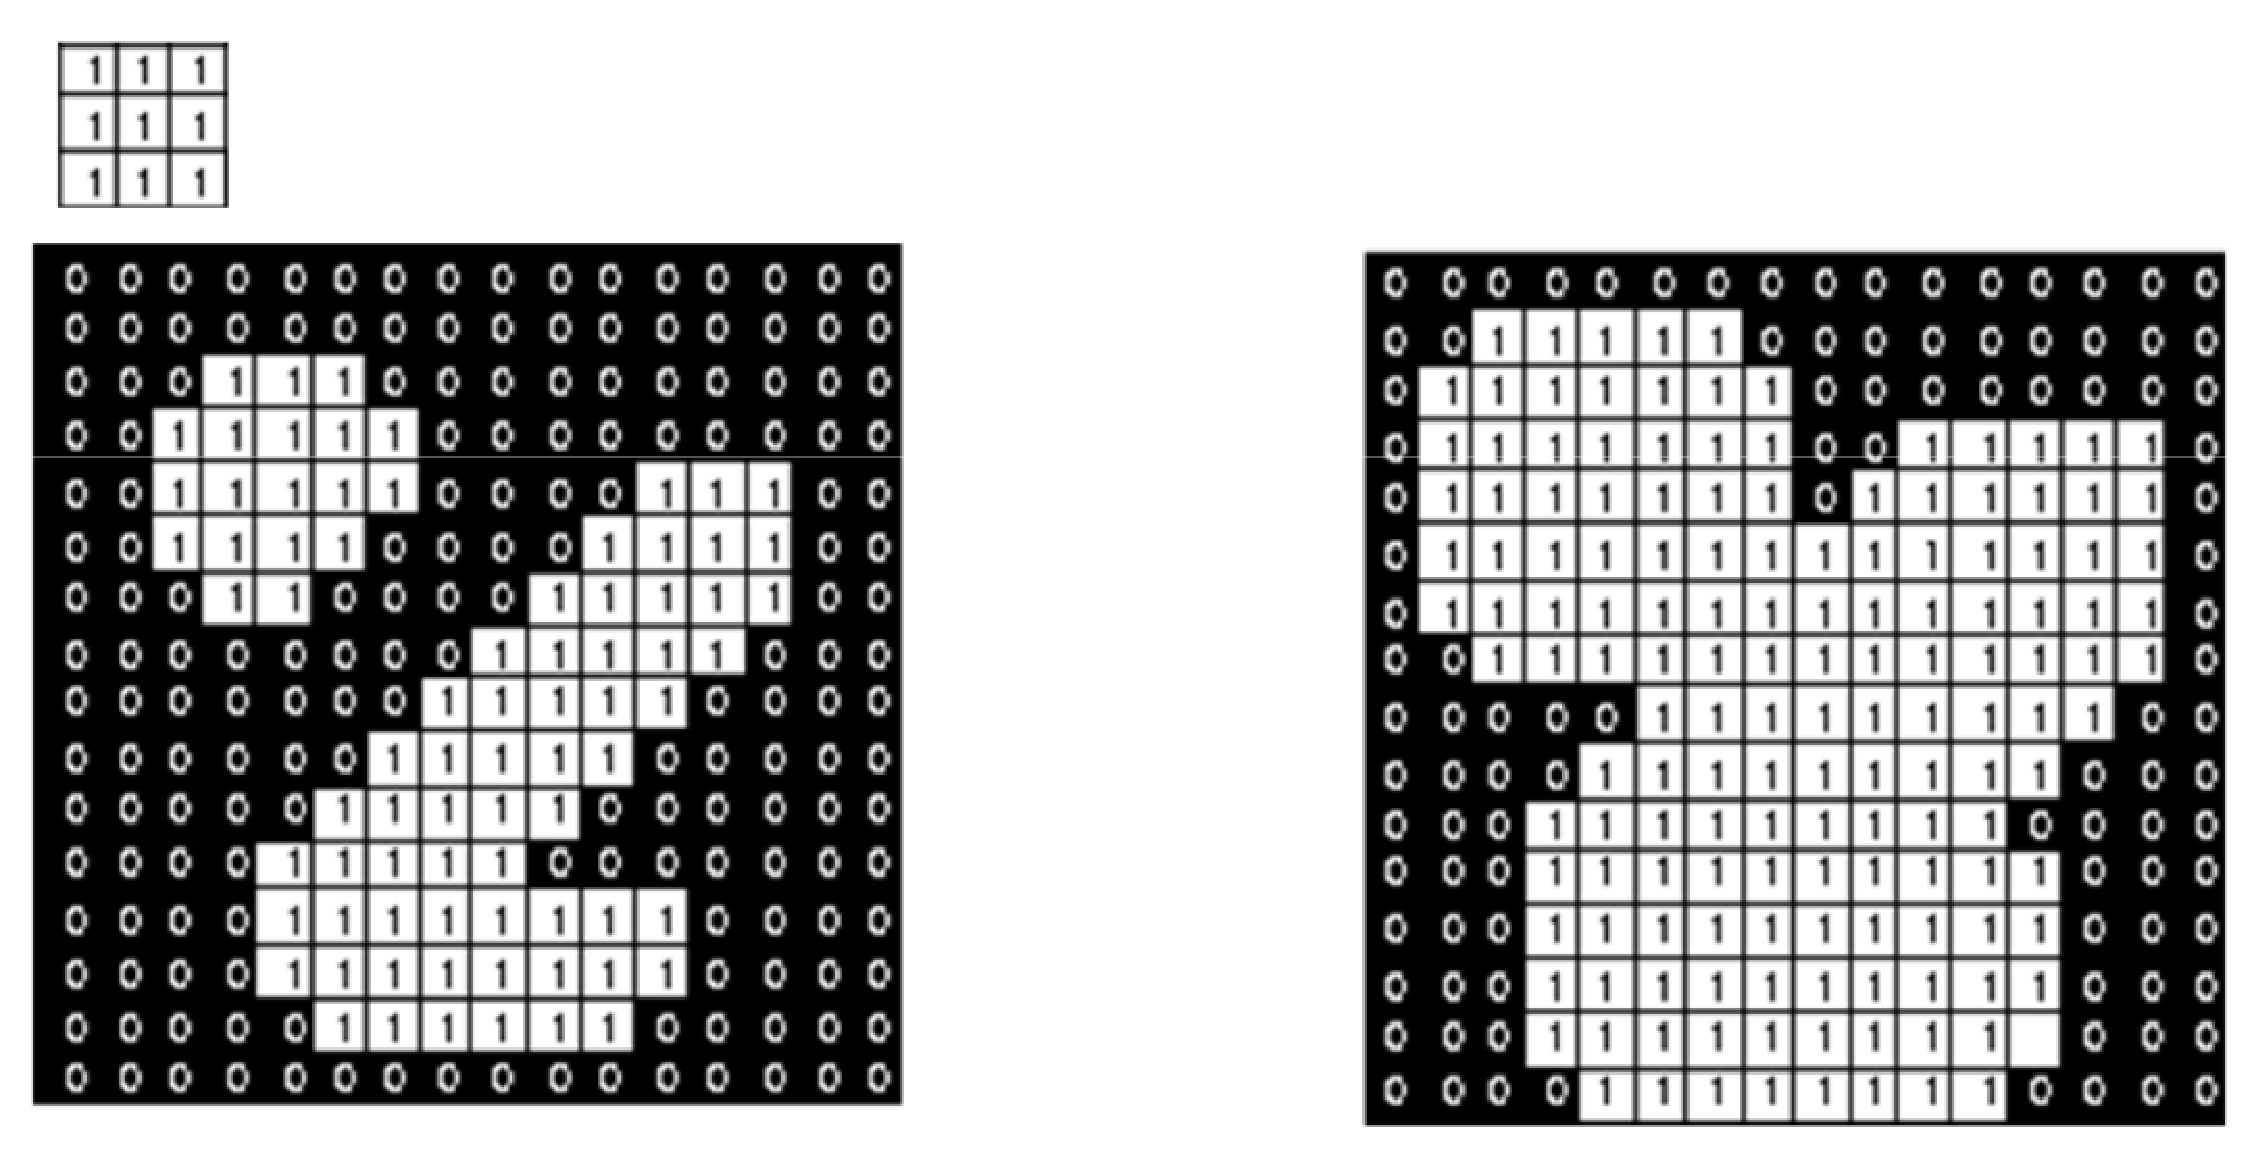
\includegraphics[width = 5 cm]{Dilatacao}
  \caption{Exemplo da opera\c{c}\~ao morfol\'ogica: Dilata\c{c}\~ao. \`A esquerda \'e a imagem original, \`a direita \'e a imagem dilatada. Fonte: fornecido pelo professor.}
  \label{fig:dilata}
\end{figure}

%%%%%%%%%%%%%%%%%%%
\subsubsection{Fechamento}
  \label{subsubsec:fechamento}
%%%%%%%%%%%%%%%%%%%
O fechamento visa suavisar contornos como, tamb\'em, funde as descontinuidades estreitas e alonga os golfos finos, elimina pequenos buracos e preenche lacunas num contorno, sendo definida como sendo:
$$ A \bullet B = [(A \oplus B) \ominus B],$$
ou seja, consiste na dilata\c{c}\~ao de $A$ por $B$, seguida da eros\~ao do resultado por $B$, como demonstrado na Figura~\ref{fig:fecha}.

\begin{figure}[!t]
  \centering
  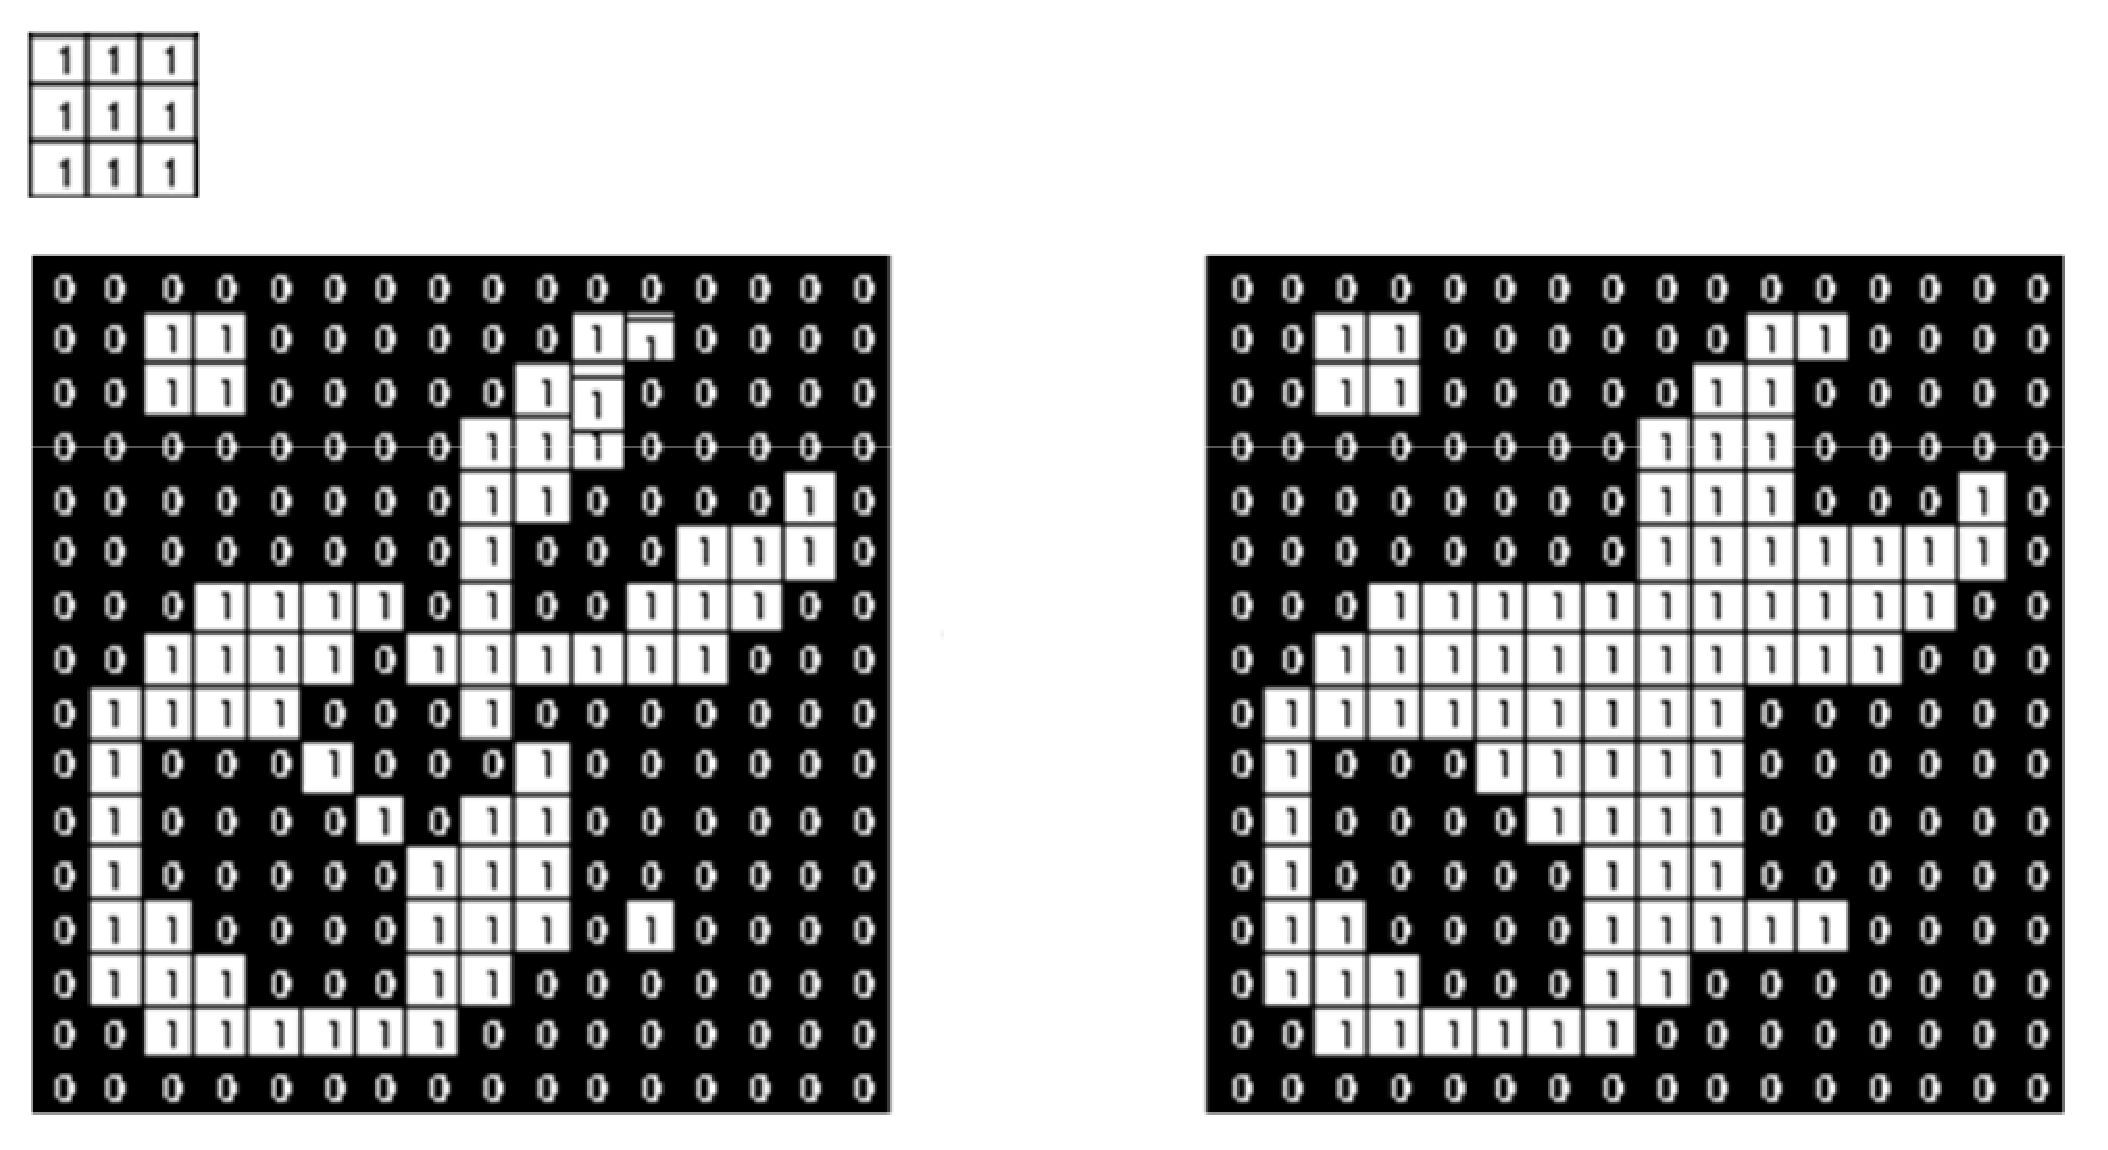
\includegraphics[width = 5 cm]{Fechamento}
  \caption{Exemplo da opera\c{c}\~ao morfol\'ogica: Fechamento. \`A esquerda \'e a imagem original, \`a direita \'e a imagem dilatada. Fonte: fornecido pelo professor.}
  \label{fig:fecha}
\end{figure}


%%%%%%%%%%%%%%%%%%%%%%%%%%%%%%%%%%%%%%%
\subsection{Segmenta\c{c}\~ao}
  \label{subsec:segmenta}
%%%%%%%%%%%%%%%%%%%%%%%%%%%%%%%%%%%%%%% 
A segmenta\c{c}\~ao consisti em dividir uma imagem em regi\~oes de interesse, de forma a permitir a extra\c{c}\~ao de suas caracter\'isticas. Para atingir este objetivo h\'a duas maneiras:~\textbf{a)} transi\c{c}\~oes, que considera as mudan\c{c}as bruscas de intensidade; ou~\textbf{b)} similaridade, que considera regi\~oes semelhantes, tendo um crit\'erio pr\'edefinido.


%%%%%%%%%%%%%%%%%%%%%%%%%%%%%%%%%%%%%%%%%%%%%%%%%%%%%%%%%%%%%%%%%%%%%%%%%%%%%
\section{Metodologia}
  \label{metodo}
%%%%%%%%%%%%%%%%%%%%%%%%%%%%%%%%%%%%%%%%%%%%%%%%%%%%%%%%%%%%%%%%%%%%%%%%%%%%%
Com as defini\c{c}\~oes feitas \'e poss\'ivel prosseguir para o desenvolvimento do projeto. Dessa forma, esta se\c{c}\~ao visa apresentar os passos seguidos para a realiza\c{c}\~ao das atividades, desenvolvidas em ~\textbf{\textit{MatLab}}~\cite{matlab}. O trabalho foi subdividido em duas partes:~\textbf{a)} detectar a m\~ao na imagem e~\textbf{b)} determinar a forma que a m\~ao assume, por isso as partes ser\~ao tratadas separadamente.

%%%%%%%%%%%%%%%%%%%%%%%%%%%%%%%%%%%%%%%
\subsection{Realce da M\~ao}
  \label{subsec:realce1}
%%%%%%%%%%%%%%%%%%%%%%%%%%%%%%%%%%%%%%%
Para o realce da m\~ao \'e considerado um par de imagem: a primeira com apenas o plano de fundo (n\~ao podendo aparecer parte do corpo); e a segunda com a m\~ao inserida no contexto. Com isso, \'e determinar a diferen\c{c}a entre as duas imagens, o que resultaria numa imagem que possui apenas a m\~ao, idealmente; mas realizando apenas a diferen\c{c}a entre as imagens foram detectados muitos ru\'idos, por isso foi realizado um incremento \`a t\'ecnica.

Ambas as imagens foram convertidas para o espa\c{c}o de cores~\textit{YCbCr}, pois as cores de pele tem maior destaque no plano~\textit{Cr}, auxiliando na segmenta\c{c}\~ao da m\~ao. Foram determinadas as diferen\c{c}as para os dois planos de cromin\^ancia, seguida pela soma das diferen\c{c}as, sendo considera como a diferen\c{c}a absoluta das imagens no espa\c{c}o de cores~\textit{YCbCr}. A difer\^en\c{c}a sobre o plano da lumin\^ancia tamb\'em foi calculada, para a determina\c{c}\~ao seu limiar de binariza\c{c}\~ao (ser\'a explicado mais adiante).

A diferen\c{c}a absoluta foi binarizada, seguido pelo processo morfol\'ogico de fechamento, pelo preenchimento de pequenos buracos e pela remo\c{c}\~ao de pequenos ru\'idos na imagem, atrav\'es da eros\~ao. Com isso, objetiva-se conseguir uma imagem com a m\~ao segmentada e alguns poucos ru\'idos. Ap\'os essas opera\c{c}\~oes, \'e realizada a detec\c{c}\~ao de regi\~oes, que servir\'a de base para o refinamento das regi\~oes, onde regi\~oes que possuem \'area total inferior a $6\%$ da \'area total da imagem s\~ao descartas, pois foi percebido que se tratavam de ru\'ido. Vale ressaltar, que  tamb\'em houveram m\~aos que foram desconsideradas nesta etapa, fruto de uma m\'a segmenta\c{c}\~ao, proporcionada pelas condi\c{c}\~oes ambientais e da c\^amera de aquisi\c{c}\~ao.

Ap\'os este processo, \'e avaliado o limiar de binariza\c{c}\~ao da diferen\c{c}a das luminosidades, citado anteriormente. Caso seja superior a $158$, significa que existia muita luminosidade, o que pode prejudicar a segmenta\c{c}\~ao da m\~ao, por isso \'e realizado o processamento, j\'a descrito, sobre a escala de cinza de ambas as imagens-base. Este procedimento \'e feito para reformar as formas gerais, pois no final \'e feita uma jun\c{c}\~ao dos resultados no espa\c{c}o de cores~\textit{YCbCr} com os da escala de cinza.

Da imagem resultante deste processamento \'e realizada a detec\c{c}\~ao de bordas, pelo m\'etodo de~\textit{Canny}~\cite{canny}, que ser\'a necess\'aria para a determina\c{c}\~ao da forma, a seguir.

%%%%%%%%%%%%%%%%%%%%%%%%%%%%%%%%%%%%%%%
\subsection{Determina\c{c}\~ao da Forma}
  \label{subsec:deterforma1}
%%%%%%%%%%%%%%%%%%%%%%%%%%%%%%%%%%%%%%%
Antes de qualquer opera\c{c}\~ao, foi analisada a orienta\c{c}\~ao da m\~ao segmentada, onde ao ser considerada como uma m\~ao na horizontal a mesma \'e invertida para a forma vertical, de forma a ter o mesmo processamento sobre todas as imagens.

Para a determina\c{c}\~ao da forma foram considerad: o bloco que engloba a m\~ao segmentada; e a imagem das bordas detectadas. Pois \'e selecionada uma linha para a realiza\c{c}\~ao de um corte horizontal na imagem, tal linha se localiza a $70\%$ da dist\^ancia do centro do bloco at\'e o topo do mesmo. Para esta linha \'e, ent\~ao, determinada a quantidade de dedos. Sobre esta linha, tamb\'em, \'e determinado a primeira e a \'ultima coluna que constitui a m\~ao.

\'E determinada, tamb\'em, uma linha m\'ovel que vai variar do centro do bloco $+15\%$ at\'e centro do bloco $-30\%$, em rela\c{c}\~ao ao topo do bloco, onde a porcentagem positiva \'e linha, visualmente, acima do centro e analogamente para a porcentagem negativa. Isto \'e feito para verificar a exist\^encia ou n\~ao de ded\~ao.

Enfim, com essas inform\c{c}\~oes a forma, que corresponde \`a m\~ao segmentada, \'e determinada. Onde s\~ao estas as escolhas:

\begin{itemize}
 \item Se houver ded\~ao, ent\~ao:
    \begin{itemize}
    \item Se dedos \'e superior a $3$, ent\~ao: Papel
    \item Sen\~ao se tiver, exatamente, $2$, ent\~ao:~\textit{Spock}
    \item Sen\~ao: Lagarto
    \item Fim\_se
    \end{itemize}
  \item Sen\~ao:
    \begin{itemize}
    \item Se dedos \'e igual a $2$, ent\~ao: Tesoura
    \item Sen\~ao:
        \begin{itemize}
	  \item Se propor\c{c}\~ao entre colunas \'e superior a limiar, ent\~ao: Pedra
	  \item Sen\~ao: Lagarto
	  \item Fim\_se
	\end{itemize}
    \item fim\_se
    \end{itemize}
  \item Fim\_se
\end{itemize}

Onde o limiar citado \'e um valor percentual da dist\^ancia entre colunas com o comprimento do bloco, equivalente a $50\%$.


%%%%%%%%%%%%%%%%%%%%%%%%%%%%%%%%%%%%%%%%%%%%%%%%%%%%%%%%%%%%%%%%%%%%%%%%%%%%%
\section{Resultados}
  \label{resut}
%%%%%%%%%%%%%%%%%%%%%%%%%%%%%%%%%%%%%%%%%%%%%%%%%%%%%%%%%%%%%%%%%%%%%%%%%%%%%
Como dito na Se\c{c}\~ao~\ref{metodo} h\'a dois problemas, dessa forma esta se\c{c}\~ao tamb\'em ser\'a subdividida. Todos os c\'odigos est\~ao dispon\'iveis~\textit{online}~\cite{down}, assim como todas as imagens-resultado obtidas com a execu\c{c}\~ao dos~\textit{scripts}. Al\'em disso, s\'o ser\~ao expostos os resultados sobre as Figuras~\ref{fig:back}, plano de fundo,~\ref{fig:mao}, plano de fundo com o acr\'escimo da m\~ao em forma de papel, e~\ref{fig:pedra}, plano de fundo com o acr\'escimo da m\~ao em forma de pedra.

\begin{figure}[]
  \centering
  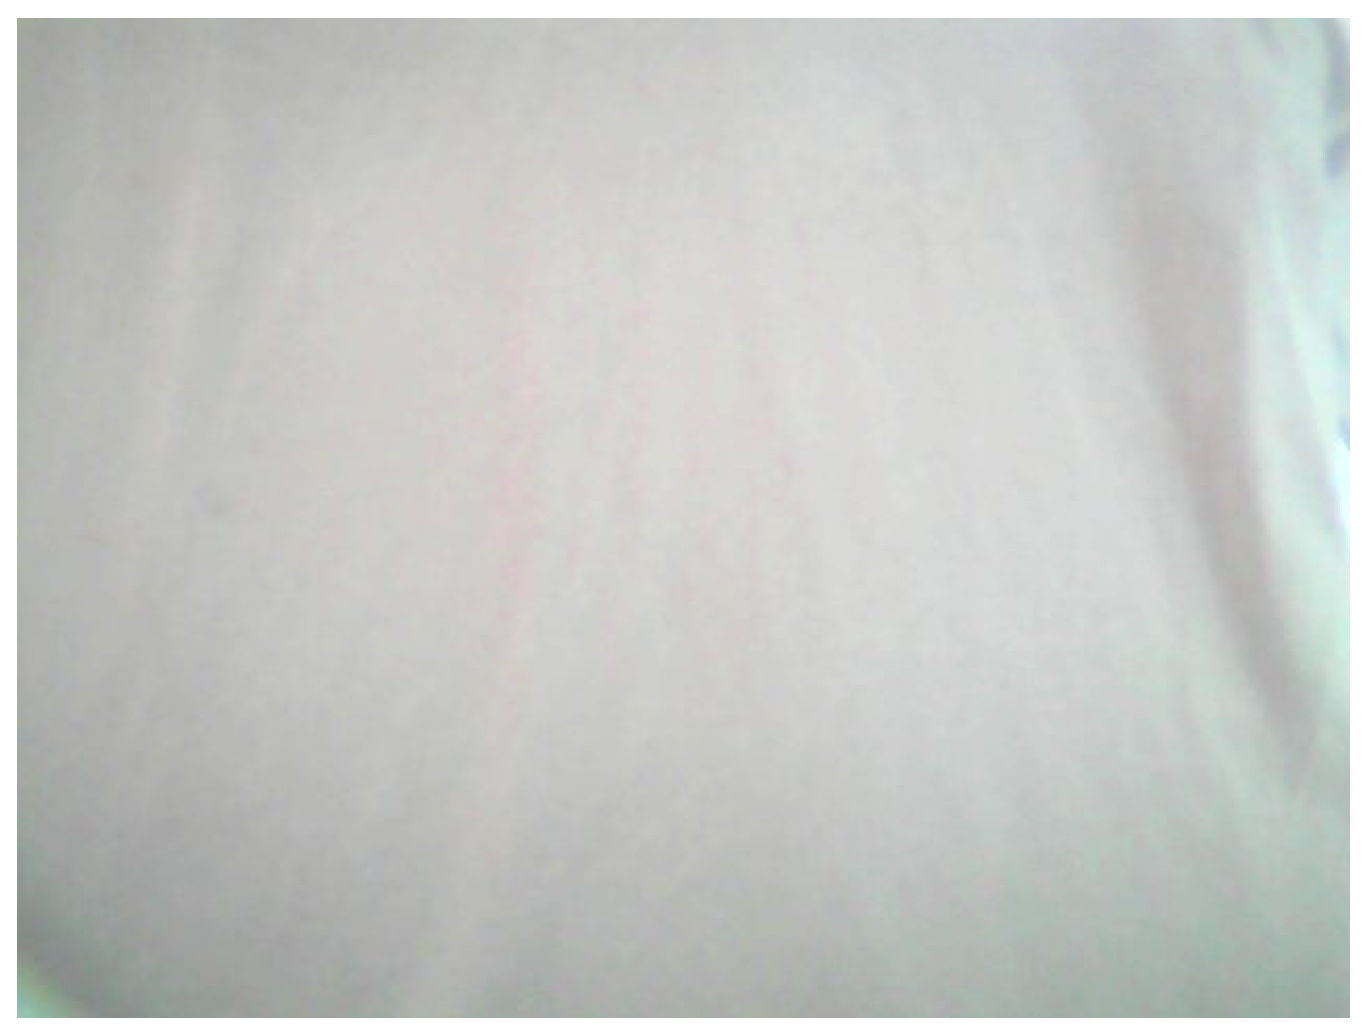
\includegraphics[width = 5 cm]{background}
  \caption{Imagem do plano de fundo considerado para exibi\c{c}\~ao dos resultados.}
  \label{fig:back}
\end{figure}

\begin{figure}[]
  \centering
  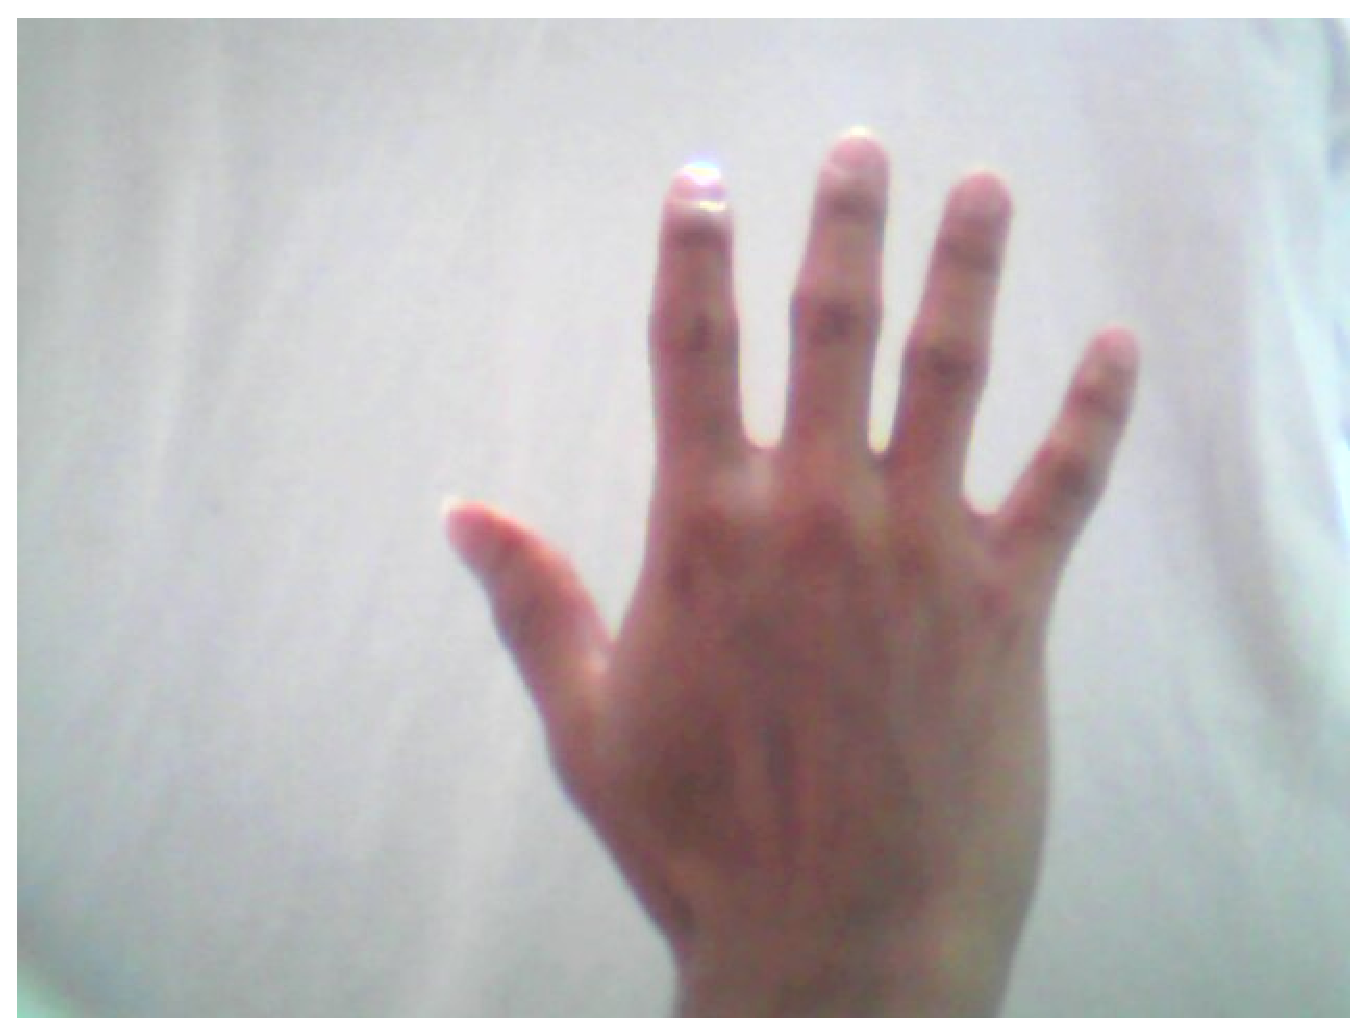
\includegraphics[width = 5 cm]{papel}
  \caption{Imagem do plano de fundo com o acr\'escimo da m\~ao, em forma de papel, considerado para exibi\c{c}\~ao dos resultados positivos.}
  \label{fig:mao}
\end{figure}

\begin{figure}[]
  \centering
  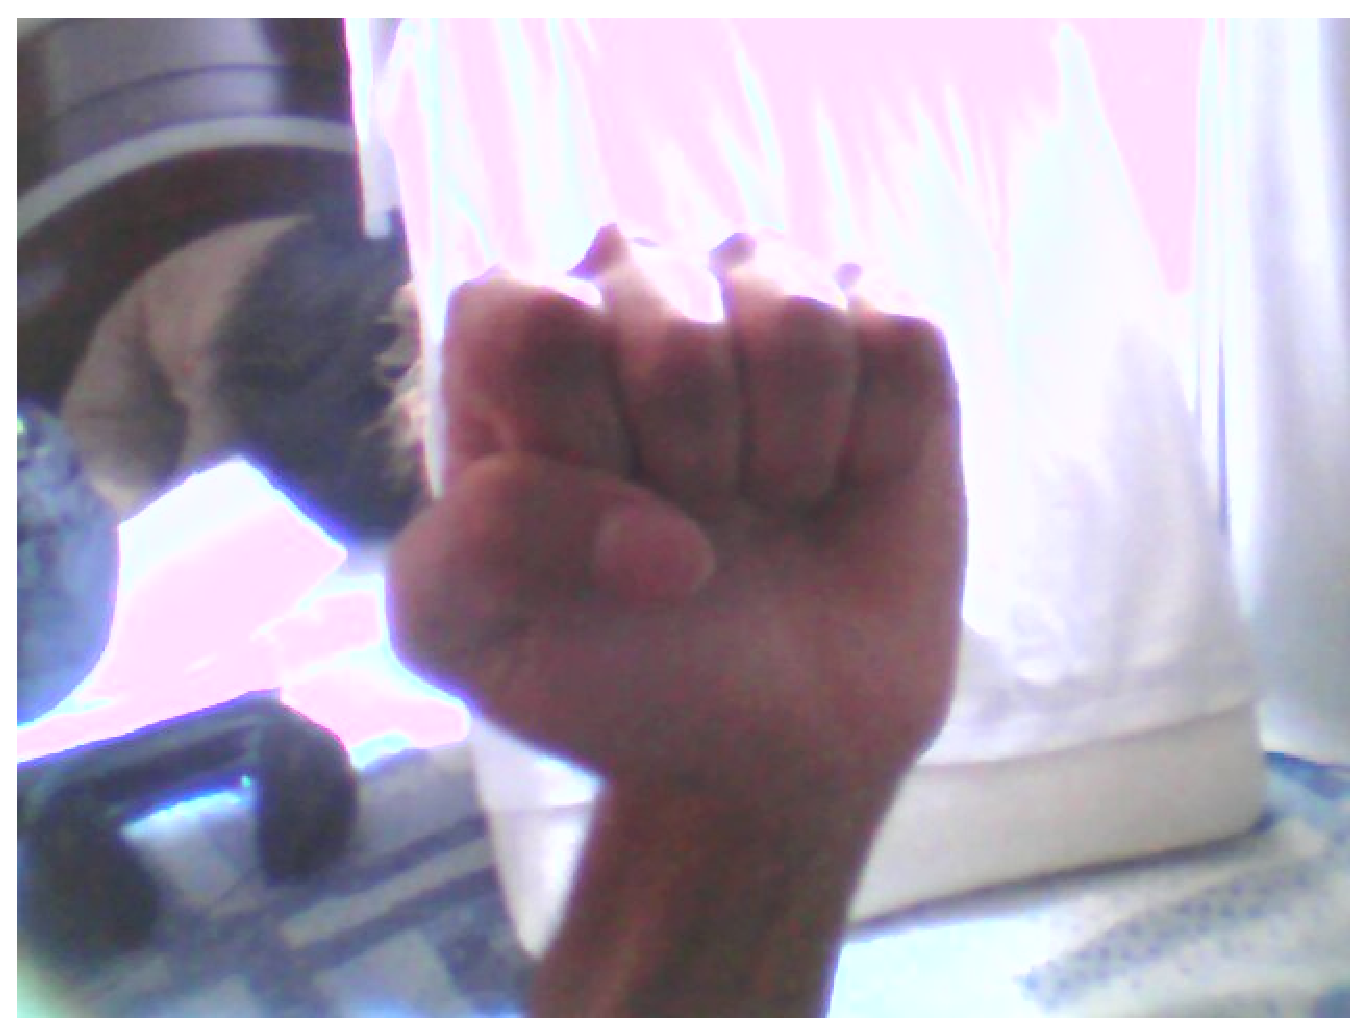
\includegraphics[width = 5 cm]{pedra}
  \caption{Imagem do plano de fundo com o acr\'escimo da m\~ao, em forma de pedra, considerado para exibi\c{c}\~ao dos resultados negativos.}
  \label{fig:pedra}
\end{figure}

%%%%%%%%%%%%%%%%%%%%%%%%%%%%%%%%%%%%%%%
\subsection{Realce da M\~ao}
  \label{subsec:realce1}
%%%%%%%%%%%%%%%%%%%%%%%%%%%%%%%%%%%%%%%
Considerando as imagens-base j\'a citadas, foi realizada a opera\c{c}\~ao de diferen\c{c}a entre os planos, o que resultou na Figura~\ref{fig:bin_dif_ycbcr} como sendo a diferen\c{c}a absoluta no espa\c{c}o de cores~\textit{YCbCr}, ap\'os a binariza\c{c}\~ao. Nesta imagem \'e poss\'ivel ver que h\'a muitas regi\~oes brancas que n\~ao correspondem a m\~ao. Por isso, tem a Figura~\ref{fig:bin_ref} como o resultado da eros\~ao, seguida pelo preenchimento de buracos e refinamento por \`area de regi\~ao, n\~ao foi preciso analisar em escala de cinza. Por fim, tem-se a Figura~\ref{fig:canny} que demonstra a decte\c{c}\~ao de borda aplicada sobre a Figura~\ref{fig:bin_ref}. Enquanto que sobre a Figura~\ref{fig:pedra} foram obtidas as Figuras~\ref{fig:bin_dif_ycbcr2},~\ref{fig:bin_ref2} e~\ref{fig:canny2}, an\'alogo ao j\'a apresentado.

\begin{figure}[]
  \centering
  
\includegraphics[width = 5 cm]{bin_dif_ycbcr}
  \caption{Resultado da binariza\c{c}\~ao sobre a imagem da diferen\c{c}a absoluta no espa\c{c}o de cores~\textit{YCbCr} da Figura~\ref{fig:mao}.}
  \label{fig:bin_dif_ycbcr}
\end{figure}

\begin{figure}[]
  \centering
  
\includegraphics[width = 5 cm]{bin_ref}
  \caption{Resultado do refinamento finalizado sobre a Figura~\ref{fig:bin_dif_ycbcr}.}
  \label{fig:bin_ref}
\end{figure}

\begin{figure}[]
  \centering
  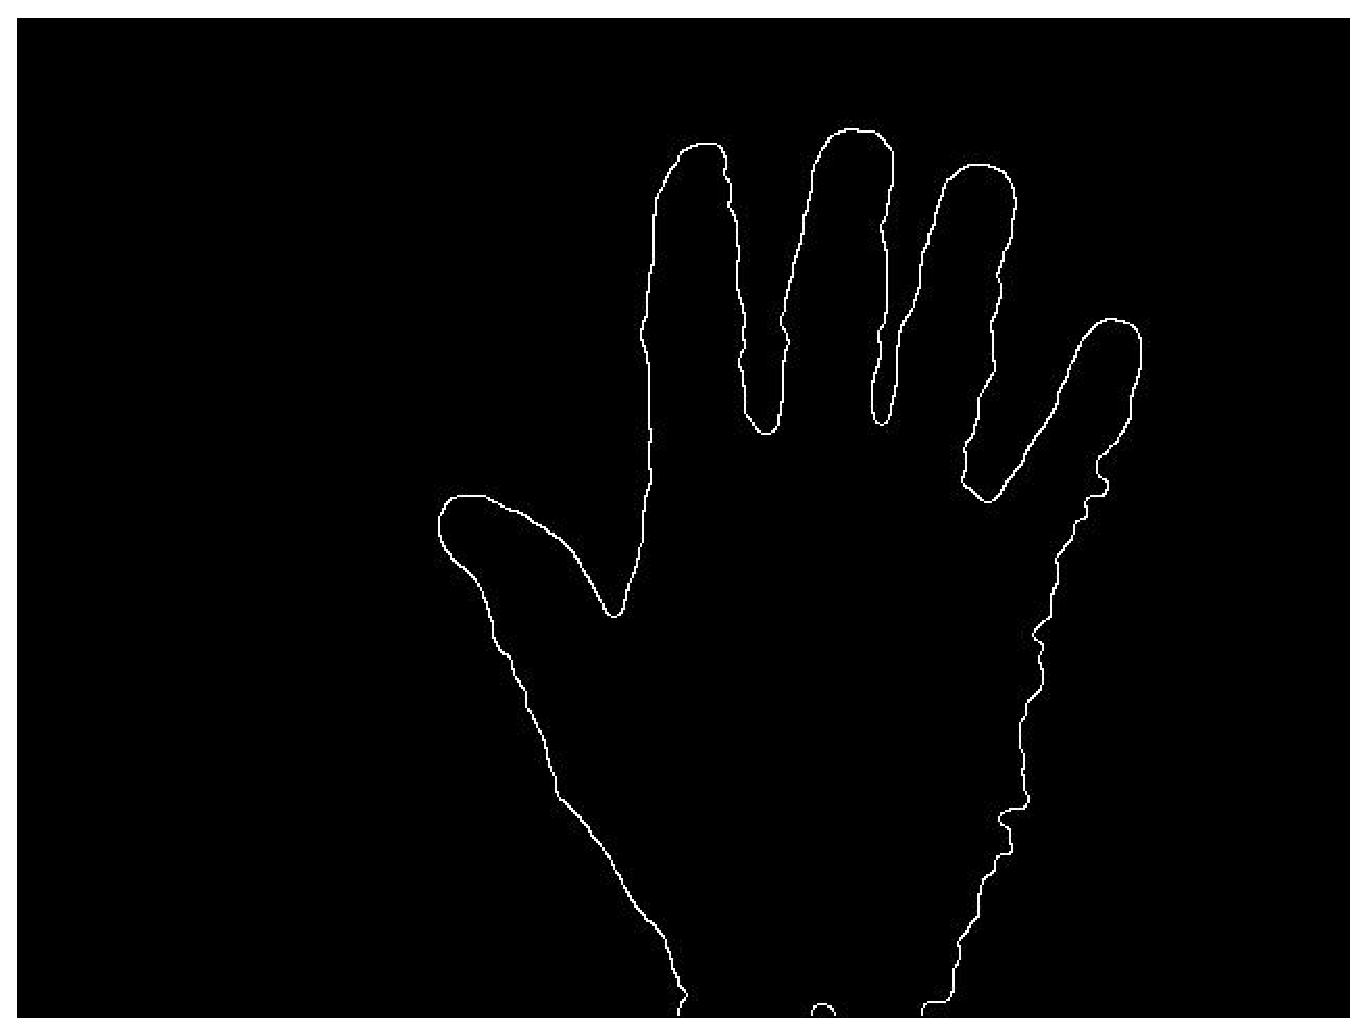
\includegraphics[width = 5 cm]{canny}
  \caption{Resultado da detec\c{c}\~ao de borda sobre a Figura~\ref{fig:bin_ref}.}
  \label{fig:canny}
\end{figure}


\begin{figure}[]
  \centering
  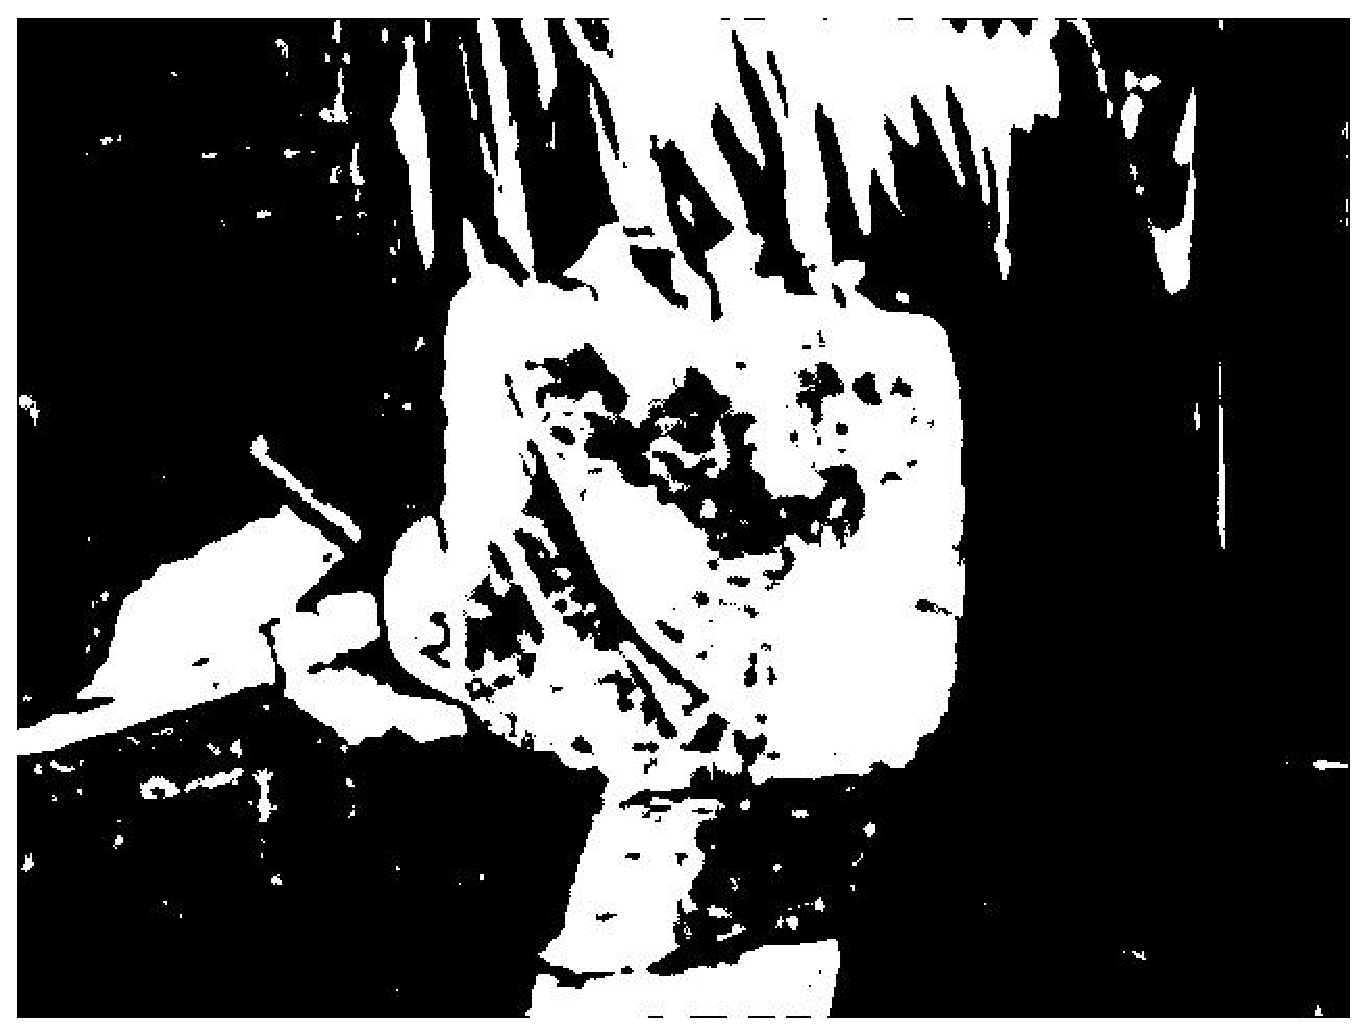
\includegraphics[width = 5 cm]{bin_dif_ycbcr2}
  \caption{Resultado da binariza\c{c}\~ao sobre a imagem da diferen\c{c}a absoluta no espa\c{c}o de cores~\textit{YCbCr} da Figura~\ref{fig:pedra}.}
  \label{fig:bin_dif_ycbcr2}
\end{figure}

\begin{figure}[]
  \centering
  
\includegraphics[width = 5 cm]{bin_ref2}
  \caption{Resultado do refinamento finalizado sobre a Figura~\ref{fig:bin_dif_ycbcr2}.}
  \label{fig:bin_ref2}
\end{figure}

\begin{figure}[]
  \centering
  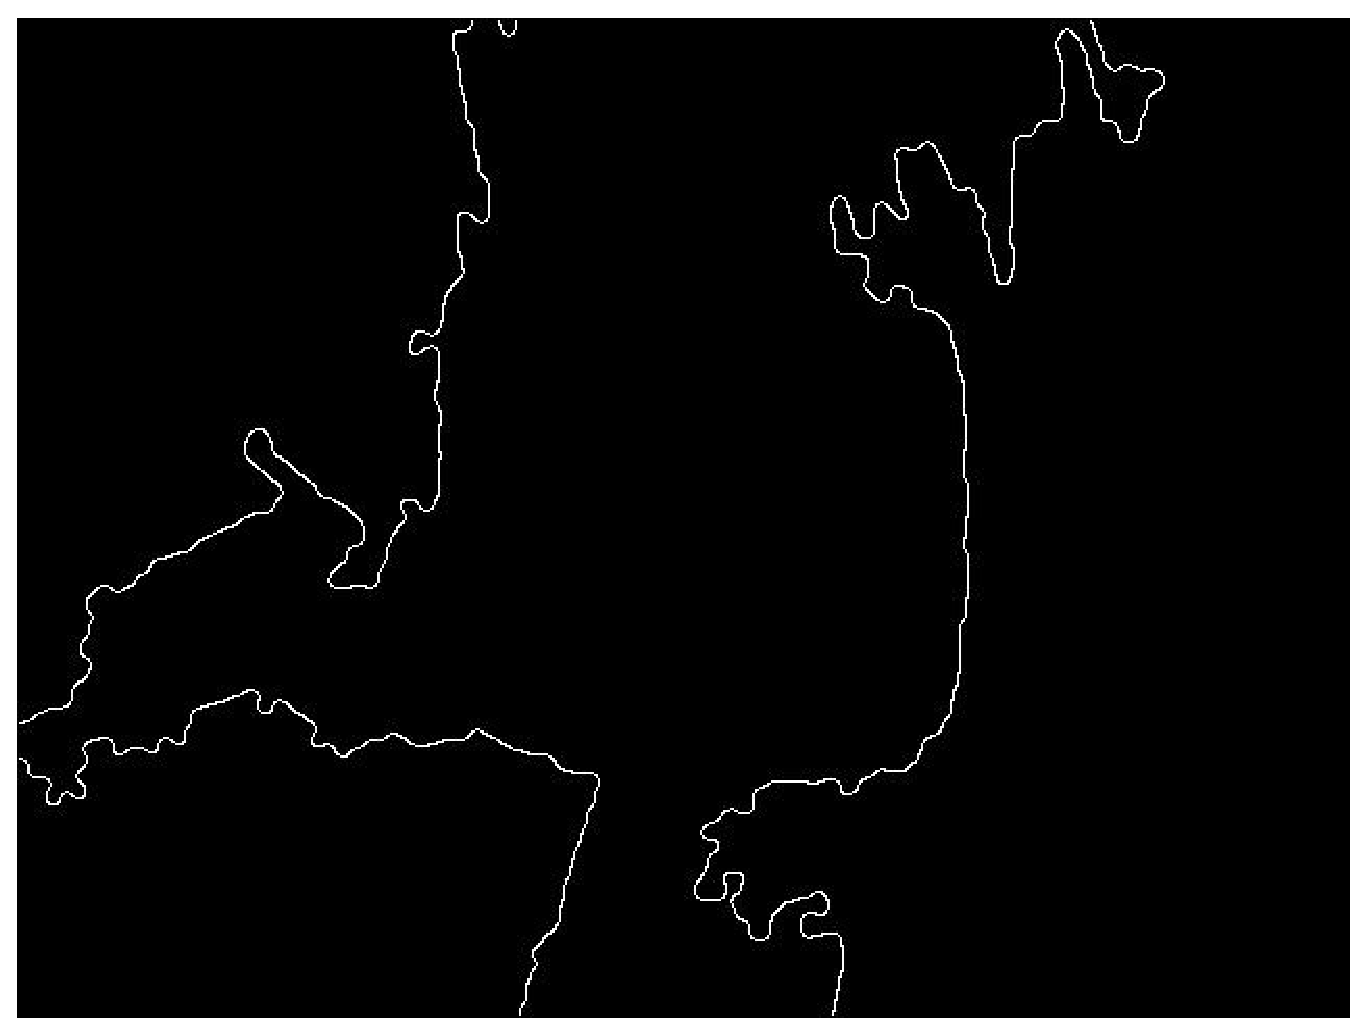
\includegraphics[width = 5 cm]{canny2}
  \caption{Resultado da detec\c{c}\~ao de borda sobre a Figura~\ref{fig:bin_ref2}.}
  \label{fig:canny2}
\end{figure}

%%%%%%%%%%%%%%%%%%%%%%%%%%%%%%%%%%%%%%%
\subsection{Determina\c{c}\~ao da Forma}
  \label{subsec:deterforma1}
%%%%%%%%%%%%%%%%%%%%%%%%%%%%%%%%%%%%%%%
A partir da Figura~\ref{fig:canny} apenas o bloco que envolve a forma foi considerado. A Figura~\ref{fig:dedos} demonstra a \`area de interesse da imagem. Dentro deste bloco foi determinado o n\'umero de dedos levantados, que para tal imagem corresponde a $3$. Ap\'os isso, foi determinado, tamb\'em, se havia ou n\~ao ded\~ao na imagem, sendo que para esta foi detectado que havia ded\~ao na imagem. Enquanto que para a Figura~\ref{fig:canny2} foi obtida a Figura~\ref{fig:dedos2}, foram detectados $2$ dedos e que tem ded\~ao.

\begin{figure}[]
  \centering
  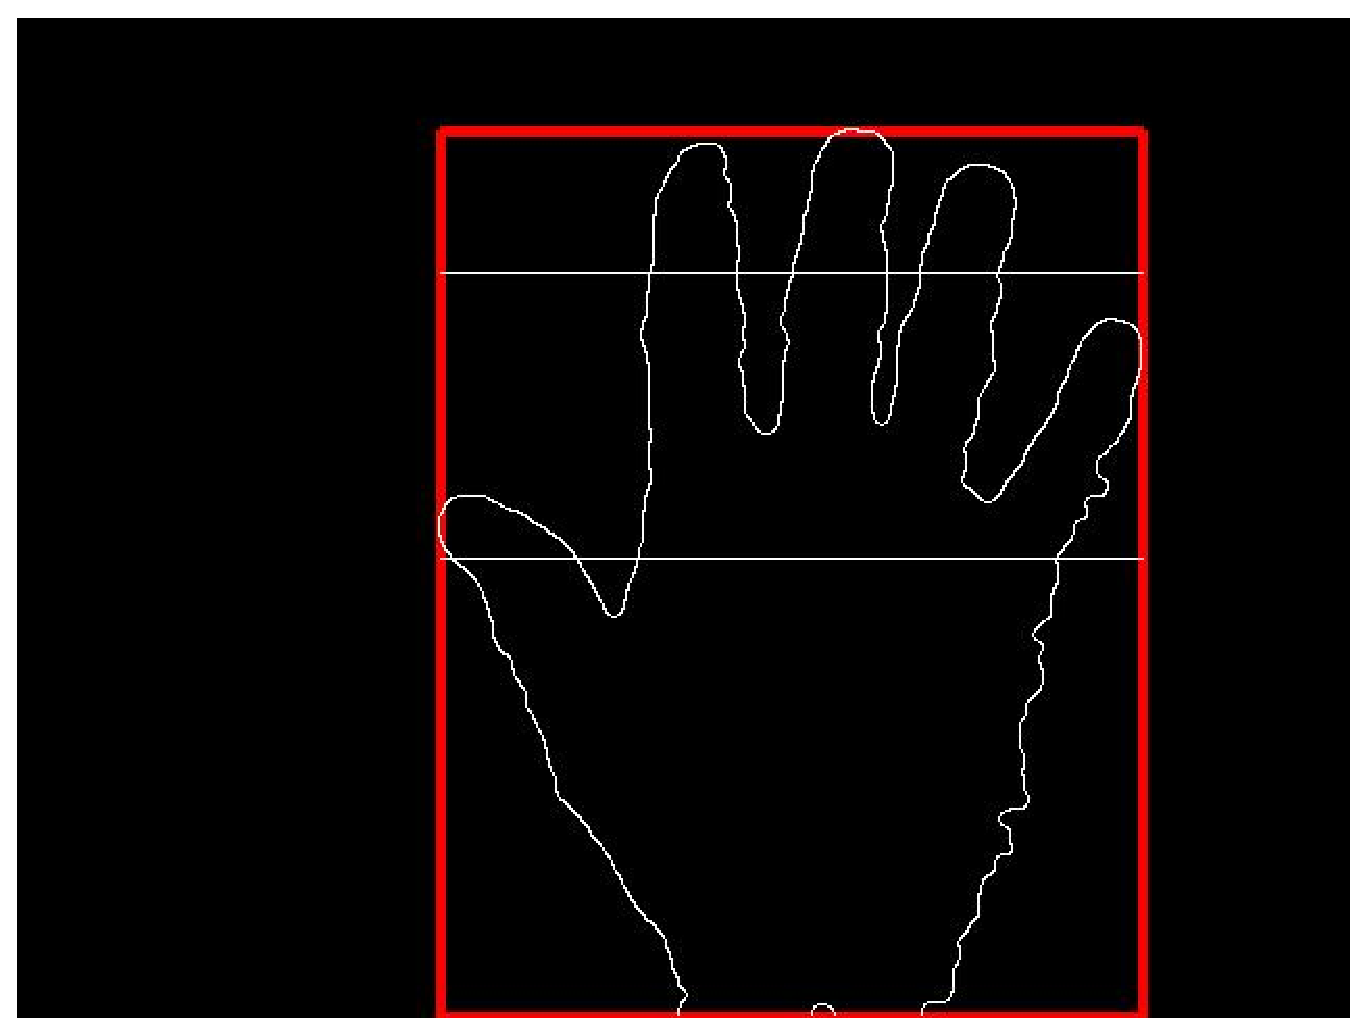
\includegraphics[width = 5 cm]{dedos}
  \caption{Bloco de interesse sobre a an\'alise da forma da m\~ao, em vermelho. A linha branca superior \'e o resultado do corte horizontal, para a detec\c{c}\~ao da quantidade de dedos levantados; j\'a a inferior \'e resultado do corte horizontal, para a detec\c{c}\~ao de ded\~ao na imagem.}
  \label{fig:dedos}
\end{figure}

\begin{figure}[]
  \centering
  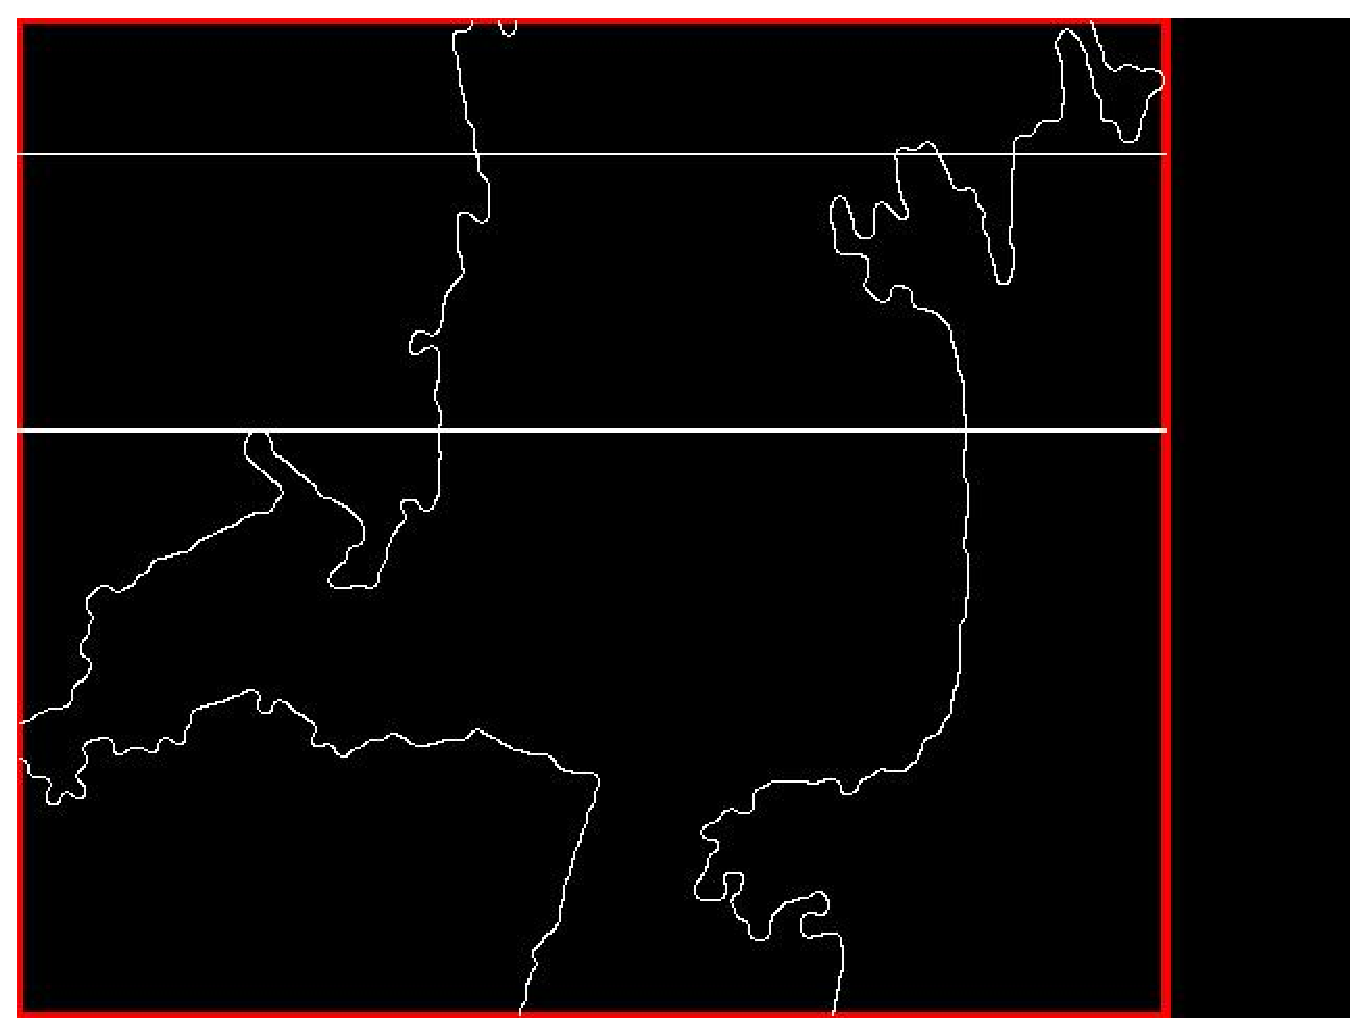
\includegraphics[width = 5 cm]{dedos2}
  \caption{Bloco de interesse sobre a an\'alise da forma da m\~ao, em vermelho. A linha branca superior \'e o resultado do corte horizontal, para a detec\c{c}\~ao da quantidade de dedos levantados; j\'a a inferior \'e resultado do corte horizontal, para a detec\c{c}\~ao de ded\~ao na imagem.}
  \label{fig:dedos2}
\end{figure}

Foram consideradas $75$ imagens para cada forma de m\~ao possivel, ou seja $227$ imagens de teste, com dois tipos de planos de fundo e mudan\c{c}as na orienta\c{c}\~ao da m\~ao. A partir dos resultados, foi constru\'ida uma estat\'istica sobre o desempenho do projeto, originando a Figura~\ref{fig:estats}. \'E poss\'ivel perceber nesta imagem que h\'a c\'elulas com cores diferenciadas, onde: vermelho significa a menor estat\'istica; e o resto em azul.

\begin{figure}[]
  \centering
  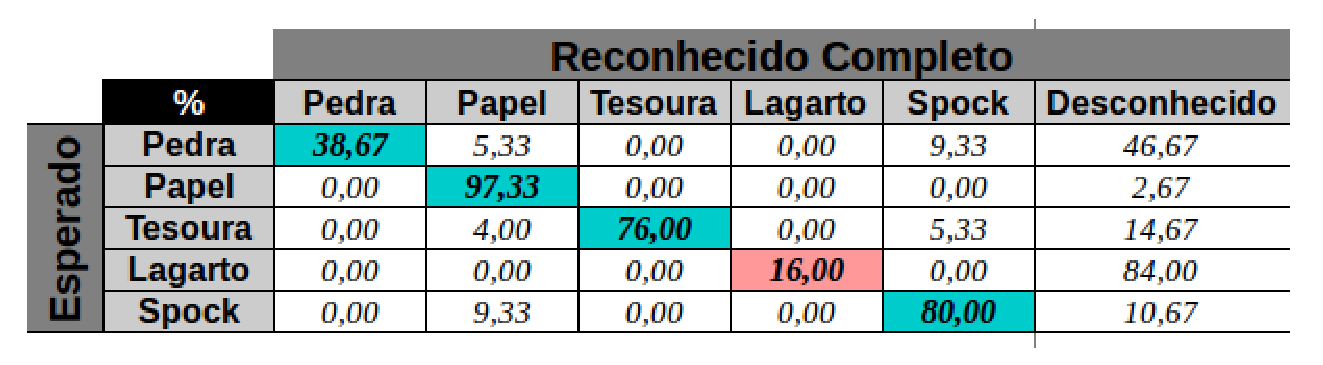
\includegraphics[width = 9 cm]{Estatisticas}
  \caption{Estat\'isticas geradas sobre o aproveitamento do projeto.}
  \label{fig:estats}
\end{figure}


%%%%%%%%%%%%%%%%%%%%%%%%%%%%%%%%%%%%%%%%%%%%%%%%%%%%%%%%%%%%%%%%%%%%%%%%%%%%%
\section{Conclus\~ao}
  \label{conclusao}
%%%%%%%%%%%%%%%%%%%%%%%%%%%%%%%%%%%%%%%%%%%%%%%%%%%%%%%%%%%%%%%%%%%%%%%%%%%%%
Com o desenvolvimento do projeto foi poss\'ivel refor\c{c}ar os conte\'udos te\'oricos visto em sala, demonstrando que o objetivo principal foi alcan\c{c}ado. Foram utilizadas as ferramentas disponibilizadas pelo~\textit{MatLab}, que possuem grande poder de atua\c{c}\~ao no processamento de imagens, o que facilitou a fixa\c{c}\~ao dos conceitos, mas \'e esperado que futuramente seja feita uma aplica\c{c}\~ao em~\textit{\textbf{OpenCV}}~\cite{opencv}~(\textit{Open Source Computer Vision Library} ou, em portugu\^es, Biblioteca de Vis\~ao Computacional em C\'odigo Aberto), assim como uma implementa\c{c}\~ao de interface gr\'afica, j\'a inicializada, mas n\~ao concluida.

O resultado do projeto foi bastante satisfat\'orio, pois foram refor\c{c}ados os t\'opicos apresentados ao longo do semestre. Al\'em disso, \'e poss\'ivel perceber, ao considerar as estat\'isticas, que o m\'etodo apresentado possui um aproveitamento mediano, pois $2/5$ das porcentagens foram acima de $80\%$, a terceira maior foi pr\'oximo deste valor e, infelizmente, a pedra e o lagarto obteveram os piores aproveitamentos. Foram encontrados problemas na segmenta\c{c}\~ao, principalmente para o lagarto, o que influ\^enciou na baixa de alguns \'indices.

Venho por meio deste me ratificar, Rodrigo, sobre os erros dos dados estat\'isticos apresentados em sala, pois havia um par\^ametro errado durante a execu\c{c}\~ao do~\textit{script}. H\'a grande varia\c{c}\~ao quanto aos resultados obtidos, o que indica que o modo de segmentar a m\~ao deve ser incrementado



% trigger a \newpage just before the given reference
% number - used to balance the columns on the last page
% adjust value as needed - may need to be readjusted if
% the document is modified later
%\IEEEtriggeratref{8}
% The "triggered" command can be changed if desired:
%\IEEEtriggercmd{\enlargethispage{-5in}}

% references section

% can use a bibliography generated by BibTeX as a .bbl file
% BibTeX documentation can be easily obtained at:
% http://www.ctan.org/tex-archive/biblio/bibtex/contrib/doc/
% The IEEEtran BibTeX style support page is at:
% http://www.michaelshell.org/tex/ieeetran/bibtex/
%\bibliographystyle{IEEEtran}
% argument is your BibTeX string definitions and bibliography database(s)
%\bibliography{IEEEabrv,../bib/paper}
%
% <OR> manually copy in the resultant .bbl file
% set second argument of \begin to the number of references
% (used to reserve space for the reference number labels box)
\begin{thebibliography}{1}

\bibitem{Gonzalez}
Gonzalez, Rafael C. e Woods, Richard E.,\emph{Digital Image Processing}, 3$^o$ ed,
Pearson Ed. - ISBN: 9780131687288. 

\bibitem{matlab}
MathWorks. \emph{MATLAB and Simulink for Technical Computing}. Dispon\'ivel em: $https://www.mathworks.com/index.html$, acessado em 2015.

\bibitem{opencv}
Documentation, OpenCV. \emph{Welcome to opencv documentation}. Dispon\'ivel em: $http://docs.opencv.org/index.html$, acessado em 2015.

\bibitem{Bruno}
Espinoza, B., Dorea, C. e Zaghetto, A. \emph{Material did\'atico utilizado em aula}.

\bibitem{Bussab}
Bussab, Wilton de Oliveira; Morettin, Pedro Alberto, \emph{Estat\'itica B\'asica}, 8$^o$ ed,
Editora Saraiva - ISBN: 9788502207998

\bibitem{down}
4Shared. \emph{Trabalho Final\_IPI}. Dispon\'ivel em:
$http://www.4shared.com/zip/IqMwwDJ8ce/TrabalhoFinal_IPI.html$.

\bibitem{rosadosventos}
Tr\'iade da Aprova\c{c}\~ao.\emph{N\'iveis de Conhecimento: Por onde come\c{c}ar e at\'e onde voc\^e deve estudar cada assunto?}. Dispon\'ivel em:
$http://triadedaaprovacao.com/niveis-de-conhecimento-por-onde-comecar-e-ate-onde-voce-deve-estudar-cada-assunto/$, acessado em 2015.

\bibitem{monitor}
One Climbs.\emph{Three: The Exploration of Archetypal Symbols Series}. Dispon\'ivel em:
$http://oneclimbs.com/2011/03/14/three-the-exploration-of-archetypal-symbols-series/$, acessado em 2015.

\bibitem{canny}
Do Vale, G. M. e Dal Poz, A. P. \emph{Processo de Detecl\c{c}ao de Bordas de Canny}. Dispon\'ivel em: $http://ojs.c3sl.ufpr.br/ojs/index.php/bcg/article/viewFile/1421/1175$, acessado em 2015.

\bibitem{jogo}
Youtube. \emph{Pedra-papel-tesoura-lagarto-Spock}. Dispon\'ivel em: $https://www.youtube.com/watch?v=abQj0pQkSOY$, acessadp em 2015.

\end{thebibliography}

% that's all folks
\end{document}